\chapter{Results}\label{sec:Results}

\section{\acs{OCV}-\acs{SOC} Curve Characterisation}
\subsection{Discharge Test}
The discharge test was conducted at a constant target current, selected so that the test duration would be compatible 
with continuous laboratory supervision, given the nominal capacity of the cell of approximately $30\,Ah$~\cite{welion2026shp270}.

\begin{equation}
    I_{dis} = \frac{30\,[Ah]}{7.5\,[h]} = 4\,[A]
\end{equation}

The discharge test was conducted with a target current of $4\,A$. The measured current profile and 
terminal voltage are shown in Figure~\ref{DischargeCurve}. The current remained approximately 
constant throughout the experiment, with an average value of $3.931\,A$ over a discharge duration of $7.019\,h$. 
The voltage profile exhibits the characteristic behaviour of a lithium-ion cell, consisting of an initial 
voltage drop followed by a gradual decrease during most of the discharge process and a steeper decline 
near the end of discharge.

\begin{figure}[H]
    \centering
    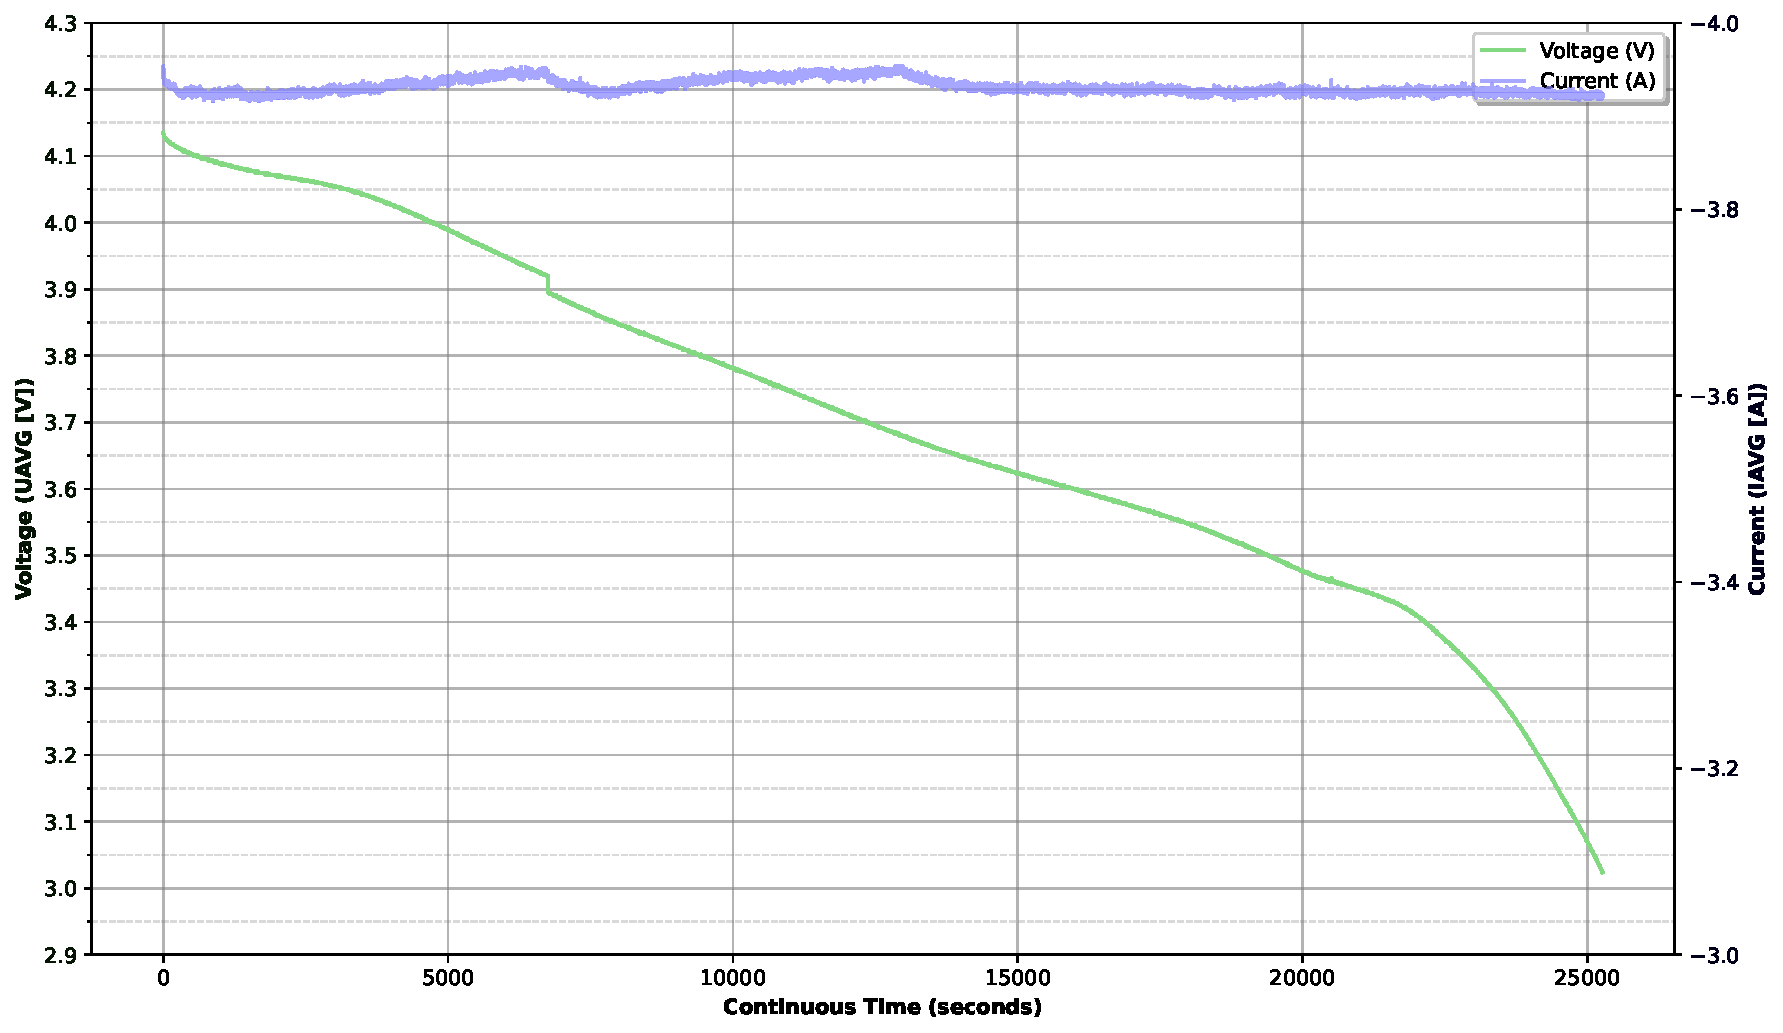
\includegraphics[width = 1\textwidth]{Codigo/Test Baterias/Battery_Graphs_Tests/Curve_Discharge_4A_3.0V_June16.pdf}
    \caption{Current (lilac) and voltage (green) curves of the \acs{NMC} battery during the discharge test.}
    \label{DischargeCurve}
\end{figure}

Although the discharge current was regulated to a constant target value, minor deviations were observed 
due to the control and measurement accuracy of the test equipment. Nevertheless, these variations were 
sufficiently small to justify the assumption of a constant current for the capacity calculation.

Using the measured average current and the total discharge duration, the actual cell capacity was 
determined as,

\begin{equation}
    Q = (3.931\,[A])(7.019\,[h]) = 27.596\,[Ah]
    \label{eq:ActualCapacityResult}
\end{equation}

The measured capacity of $27.596\,Ah$ is approximately $8.0\%$ lower than the $30\,Ah$ nominal capacity specified 
by the manufacturer. This difference may be attributed to testing conditions, cell ageing, or the 
selected discharge cut-off voltage.

The total energy delivered by the cell during the discharge test was obtained from 
the measured voltage and current data. The power analyser directly provided the accumulated 
energy in watt-seconds, which was converted to watt-hours according to the following equation,

\begin{equation}
    E_{dis} = \frac{366,982.4\,[Ws]}{3,600} = 101.939\,[Wh]
    \label{eq:EdisDiscrete}
\end{equation}

The measured discharged energy was $101.939\,Wh$, corresponding to approximately 91.8\% of the nominal 
energy rating of $111\,Wh$ specified by the manufacturer.

\subsection{Charge Test}
The charging test was performed with a maximum charging current of $20\,A$ and a total charging duration 
of $1.94\,h$. The measured voltage and current profiles are presented in Figure~\ref{ChargeCurve}. 
The results exhibit the expected \ac{CC-CV} charging behaviour of 
lithium-ion cells.

\begin{figure}[H]
    \centering
    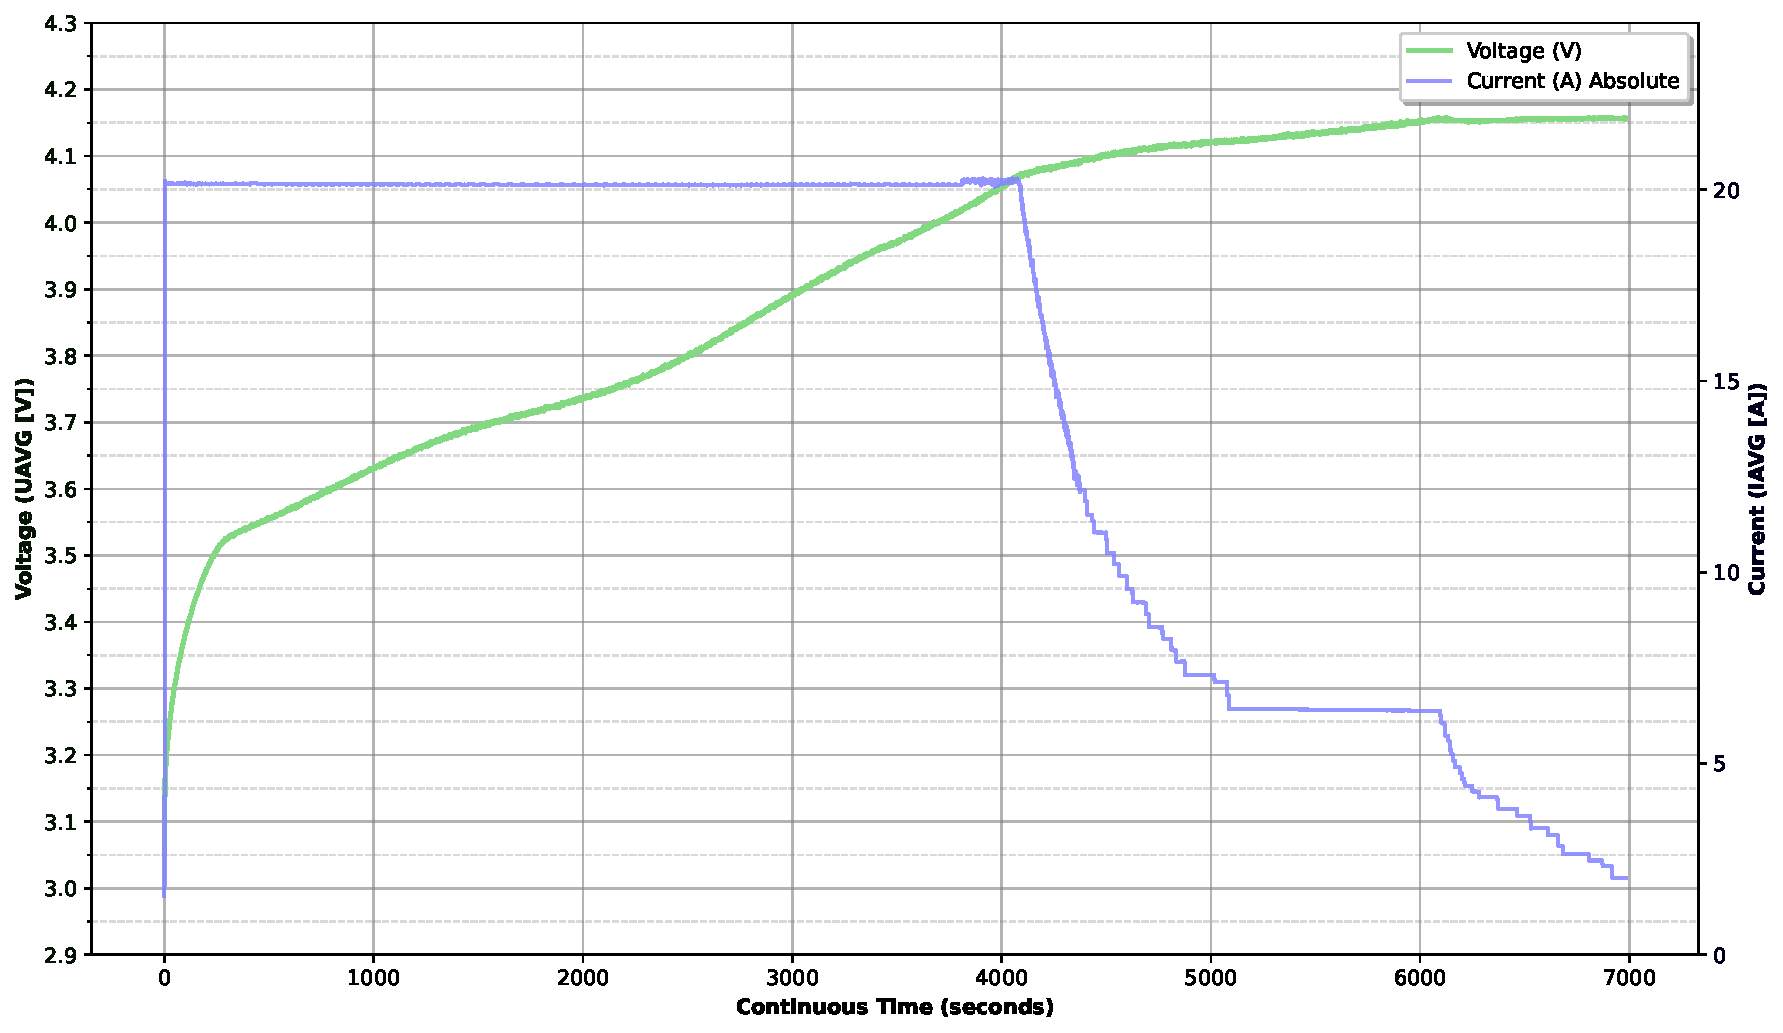
\includegraphics[width = 1\textwidth]{Codigo/Test Baterias/Battery_Graphs_Tests/Curve_Charge_20A_4.15V_Jun22.pdf}
    \caption{Current (lilac) and voltage (green) curves of the \acs{NMC} battery during the charge test.}
    \label{ChargeCurve}
\end{figure}

During the constant-current phase, the charging current remained close to $20\,A$ while the terminal 
voltage increased progressively. Once the cell voltage reached approximately $4.05\,V$, the charger 
transitioned to the constant-voltage phase, where the charging current gradually decreased and the voltage slowly increased. 
The charging process was terminated when the voltage reached $4.15\,V$, current dropped below approximately $2.009\,A$.

\begin{equation}
    E_{charge} = \frac{400,964.76\,[Ws]}{3,600} = 111.379\,[Wh]
    \label{eq:EChargeDiscrete}
\end{equation}

The total energy supplied to the battery during charging was $111.379\,Wh$. Then, the efficiency was calculated 
based on the measured this charging and discharging energies, the energy efficiency of the cell was $91.5\%$.

\begin{equation}
    \eta = (100)\frac{101.939\,[Wh]}{111.379\,[Wh]} = 91.524\%
    \label{EtaEfficiency}
\end{equation}

While the manually calculated capacity from Equation~\eqref{eq:ActualCapacityResult} was $27.596\,Ah$, 
the battery analyser's direct accumulated-Ah reading of $27.616\,Ah$ was adopted as the reference capacity for 
all subsequent parameter identification and EKF implementation, as the two values differ by less than 0.1\%.

\subsection{Pulses Test}\label{PulsesTestsResults}
The pulse-discharge test was conducted using \ac{SOC} intervals of 5\%, with a relaxation period of three 
minutes between consecutive pulses. The pulse magnitude and duration were selected such that each 
pulse removed an approximately constant amount of charge from the cell.

Using the experimentally determined capacity from Equation~\eqref{eq:ActualCapacityResult}, the charge 
corresponding to each 5\% \ac{SOC} decrement was calculated as,

\begin{equation}
    Q_{step} = (27.616\,[Ah])(5\%) = 1.3808\,[Ah]
    \label{QStep}
\end{equation}

Three discharge current levels were employed during the test. For the first eighteen \ac{SOC} intervals 
(approximately 90\% of the usable capacity), a current of $10\,A$ was used. 
As the cell approached the lower voltage region, the discharge current was reduced to $3 A$, and 
finally to $1\,A$ near the end of discharge to improve the resolution of the low \ac{SOC} measurements.

\begin{equation}
    t_{dis_{10A}} = \frac{1.3808\,[Ah]}{10\,[A]} 60 \approx 8\,[minutes]
\end{equation}

\begin{equation}
    t_{dis_{3A}} = \frac{1.3808\,[Ah]}{3\,[A]} 60 \approx 27\,[minutes]
\end{equation}

\begin{figure}[H]
    \centering
    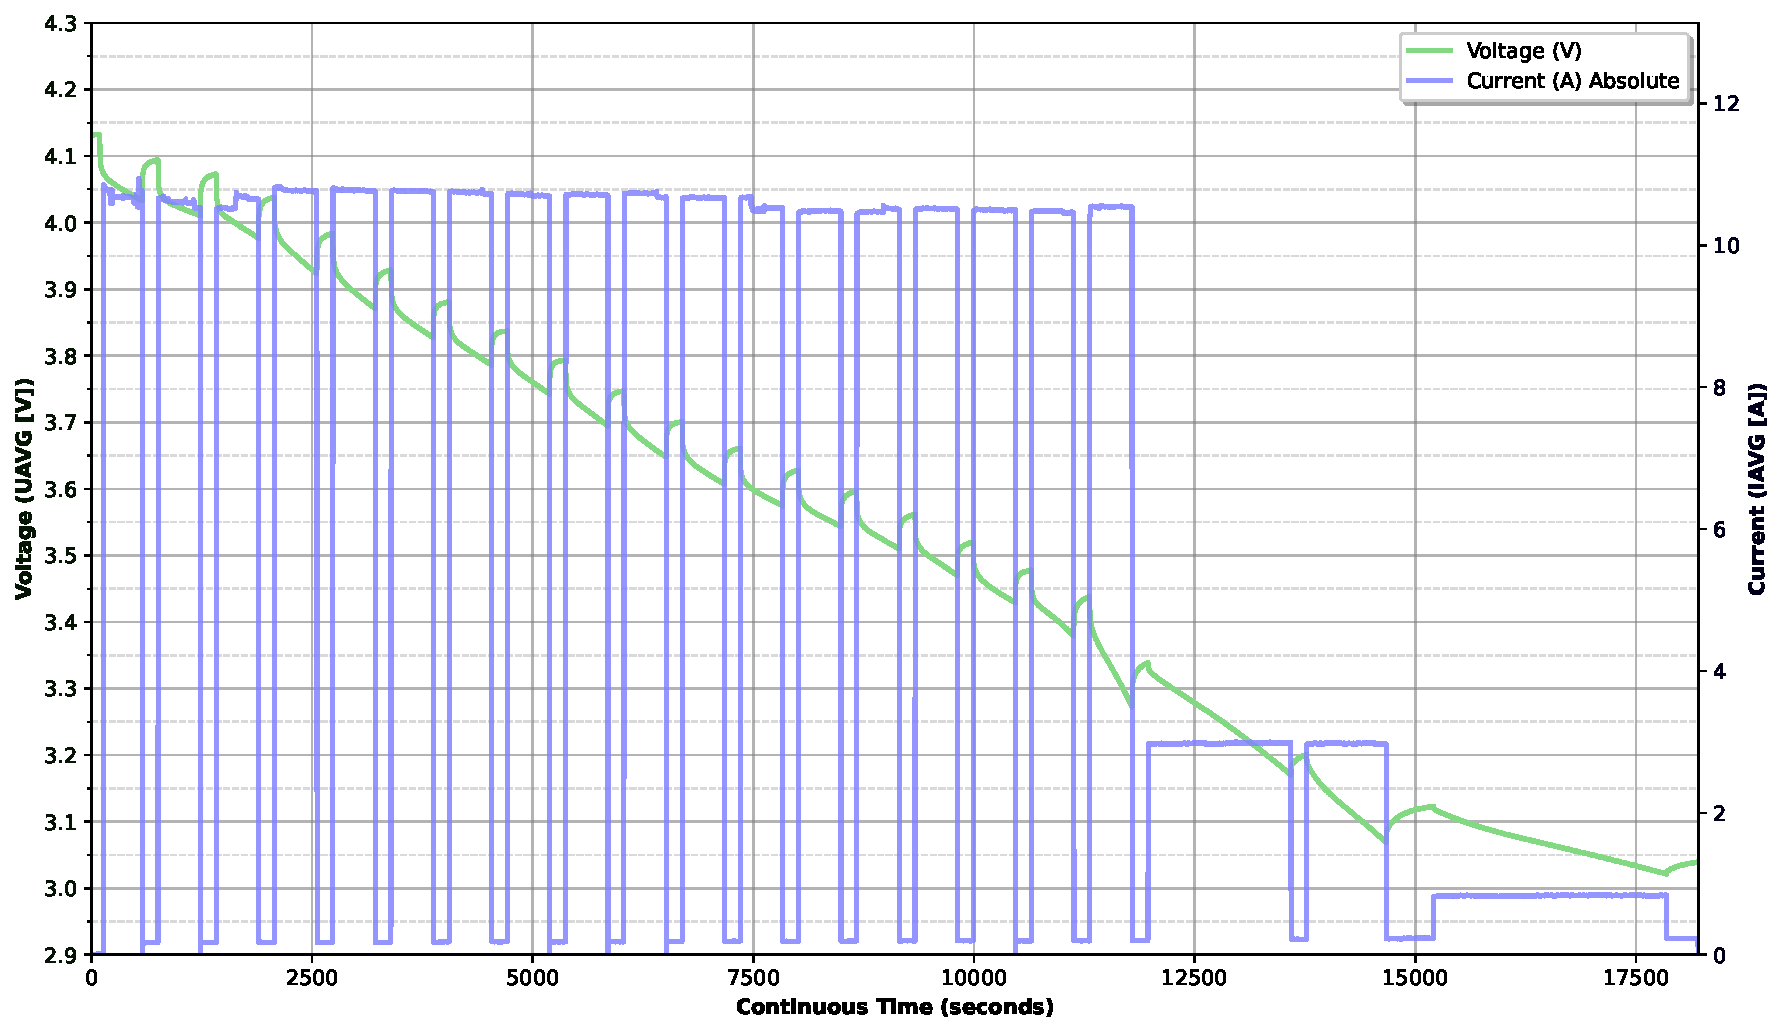
\includegraphics[width = 1\textwidth]{Codigo/Test Baterias/Battery_Graphs_Tests/PulseCurve_Pulsos_10A_3A_1A_Jun22.pdf}
    \caption{Current (lilac) and voltage (green) curves of the \acs{NMC} battery during the 
    pulses test.}
    \label{TrainOfPulsesResult}
\end{figure}

Figure~\ref{TrainOfPulsesResult} presents the complete pulse discharge test. During each current pulse, 
the terminal voltage decreases due to both the open-circuit voltage variation and the internal voltage 
drops associated with the cell impedance. 
Once the current is interrupted, the voltage partially recovers during the relaxation period and 
gradually approaches an equilibrium value.

The voltage measured at the end of each relaxation period was used as an approximation of 
the open-circuit voltage corresponding to the current \ac{SOC} level. These \ac{OCV}-\ac{SOC} pairs were subsequently 
used to construct the \ac{OCV}-\ac{SOC} relationship shown in Figure~\ref{OCV-SOCResult}.

% Figure~\ref{TrainOfPulsesResult} shows twenty one sets of pulses, where in between pulses, during the relaxation period, the
% voltage of the battery decreases until the next pulse begins. These voltage points, along with it's corresponding percentage
% of charge consititute the OCV-SOC curve presented in Figure~\ref{OCV-SOCResult}. \textcolor{red}{The max voltage corresponding
% to 100\% SOC is 4.141 V and in the other end the fully discharged battery is when voltage reaches 3.021 V}.

\begin{figure}[H]
    \centering
    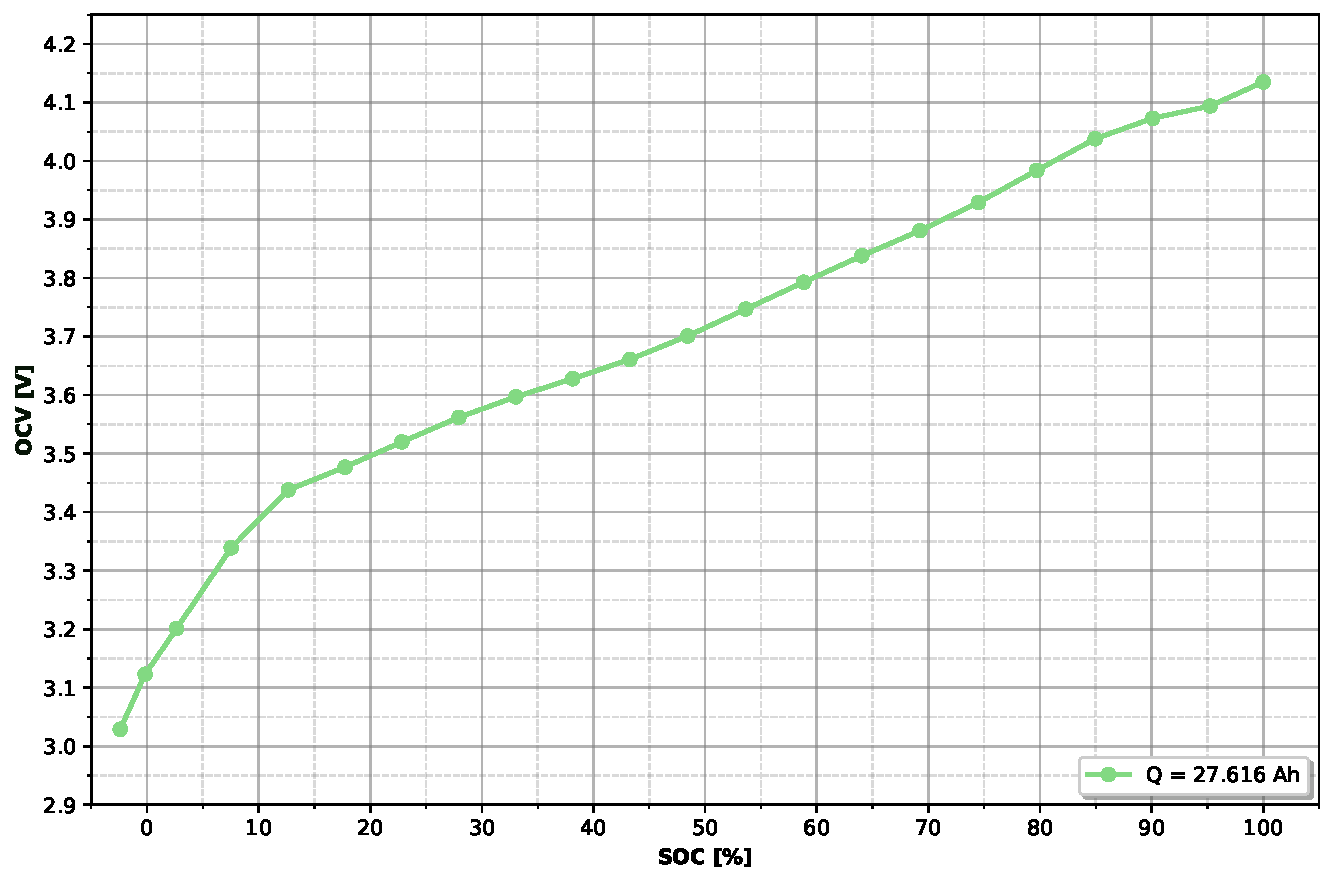
\includegraphics[width = 1\textwidth]{Codigo/Test Baterias/Battery_Graphs_Tests/OCV_SOC_curve_Qref_Pulsos_10A_3A_1A_Jun22.pdf}
    \caption{OCV-SOC curve of the \acs{NMC} battery.}
    \label{OCV-SOCResult}
\end{figure}

The resulting \ac{OCV}-\ac{SOC} curve exhibits the characteristic nonlinear behaviour of \acs{NMC} lithium-ion cells. 
The voltage varies gradually throughout the middle region, while steeper voltage gradients are observed 
near fully charged and fully discharged conditions. The measured \ac{OCV} ranged from $4.138\,V$ at 100\% SOC 
to $3.029\,V$ at 0\% SOC.

The experimentally obtained \ac{OCV}-\ac{SOC} relationship was subsequently implemented as a lookup table within 
the equivalent-circuit model and for the \ac{EKF} estimation algorithm.

\section{Parameter Identification}
\subsection{$R_0$, $R_1$, $R_2$, $C_1$, $C_2$ parameters}
The parameter identification test was performed by subjecting the cell to a two-level step-current sequence at each \ac{SOC} operating point, the first pulse was $10\,A$ for 
$90\,s$ followed immediately by a second pulse of $30\,A$ for $90\,s$, with a relaxation period of $10$ minutes between each consecutive cycle. This protocol was 
repeated until the battery reached the minimum voltage established as $3.0\,V$.
\\
The algebraic identification method~\cite{DEVARAKONDA2014} was applied to each cycle independently to extract the six equivalent-circuit parameters 
($R_0$, $R_1$, $R_2$, $C_1$, $C_2$, and the open-circuit voltage $E$). To assess the 
reliability of each identification, the extracted $E$ value was compared against the \ac{OCV}-\ac{SOC} curve established from the pulse discharge test 
shown in Section~\ref{PulsesTestsResults}. Cycles for which the deviation $|E_{\text{extracted}} - \text{OCV}(\text{SOC})|$ exceeded $20\,\text{mV}$ were 
considered numerically unreliable and excluded from the $R_1$ and $C_1$ tables. 
This criterion excluded two cycles and the remaining cycles spanned from $16.6\%$ to $99.9\%$ \ac{SOC}, which were retained for $R_1$ and $C_1$. All twelve 
cycles were used for $R_0$, $R_2$, and $C_2$, as these parameters showed consistent values across the full range.
\\
The identified resistance values are presented in Figure~\ref{ResistorsParamResult}. 
The ohmic resistance $R_0$ remained approximately constant across the \ac{SOC} range, with values between $2.1\,\text{m}\Omega$ and $2.6\,\text{m}\Omega$. The diffusion 
resistance $R_2$ also showed low variability, remaining below $1.1\,\text{m}\Omega$. The polarisation resistance $R_1$ exhibited larger variability, 
consistent with the known sensitivity of this parameter to the observation window of the algebraic method~\cite{DEVARAKONDA2014}, and is discussed 
further in Section~\ref{sec:Conclusion}.

\begin{figure}[H]
    \centering
    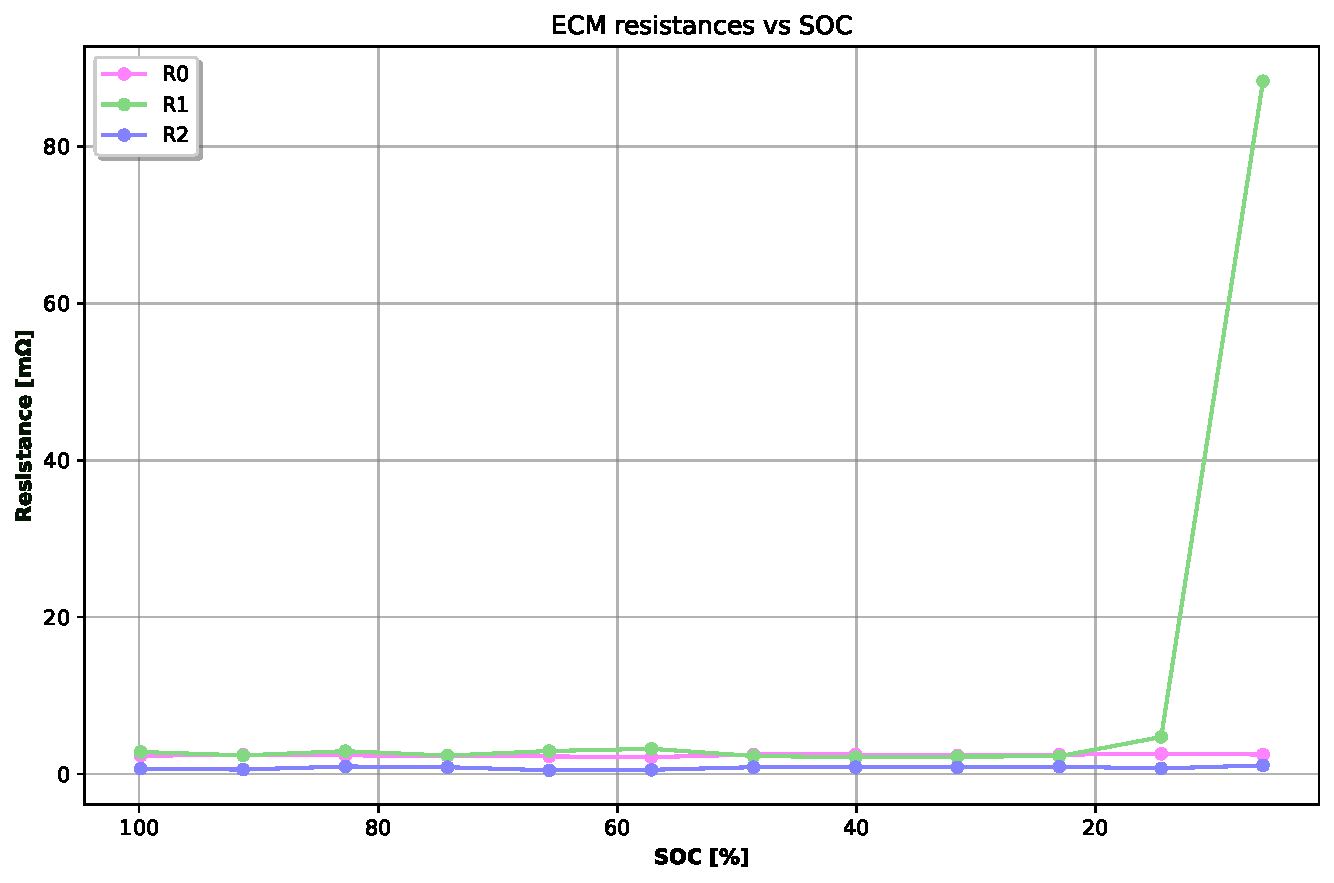
\includegraphics[width = 1\textwidth]{Codigo/Test Baterias/Battery_Graphs_Tests/ECM_resistances_vs_SOC_Param_0A_10A_30A_Jun30.pdf}
    \caption{Resistors $R_0$ (pink), $R_1$ (green), and $R_2$ (lilac) values of the \acs{NMC} battery.}
    \label{ResistorsParamResult}
\end{figure}

The capacitance values, shown in Figure~\ref{CapacitorsParamResult} on a logarithmic scale, ranged from approximately $18,000\,\text{F}$ to $33,000\,\text{F}$ for $C_1$ 
and from $4,000\,\text{F}$ to $13,000\,\text{F}$ for $C_2$ across the \ac{SOC} points.

\begin{figure}[H]
    \centering
    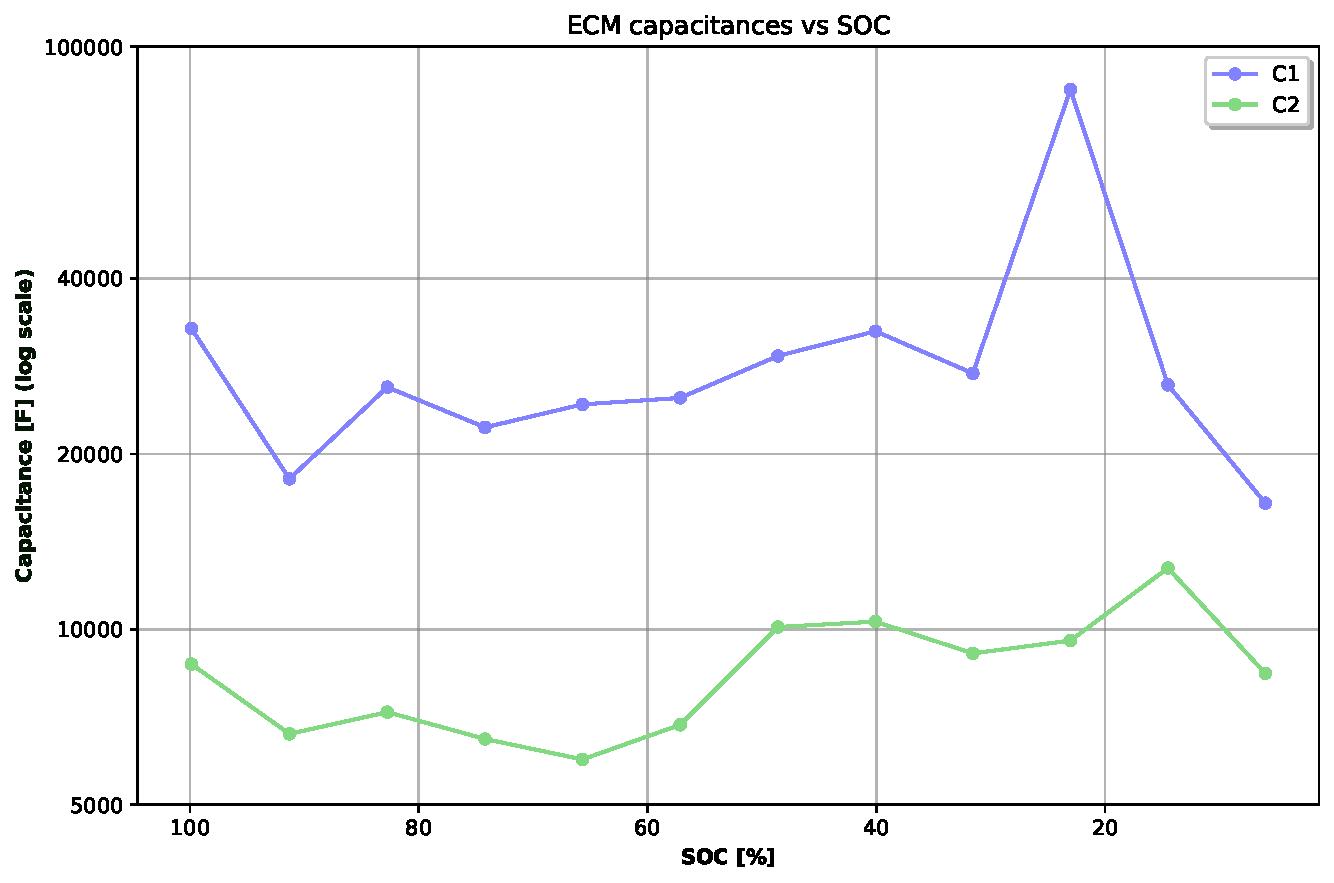
\includegraphics[width = 1\textwidth]{Codigo/Test Baterias/Battery_Graphs_Tests/ECM_capacitances_vs_SOC_Param_0A_10A_30A_Jun30.pdf}
    \caption{Capacitors $C_1$ (lilac) and $C_2$ (green) values of the \acs{NMC} battery.}
    \label{CapacitorsParamResult}
\end{figure}

Figure~\ref{ECurveParamResult} presents a comparison between the \ac{OCV}--\ac{SOC} curve obtained from the pulse discharge test and the $E$ values extracted from the 
parameter identification cycles. The two curves show similar behaviour across the middle \ac{SOC} range, confirming the consistency of the parameter identification 
procedure. The mean absolute deviation between the two curves, computed over the ten validated cycles, was below $10\,\text{mV}$.

\begin{figure}[H]
    \centering
    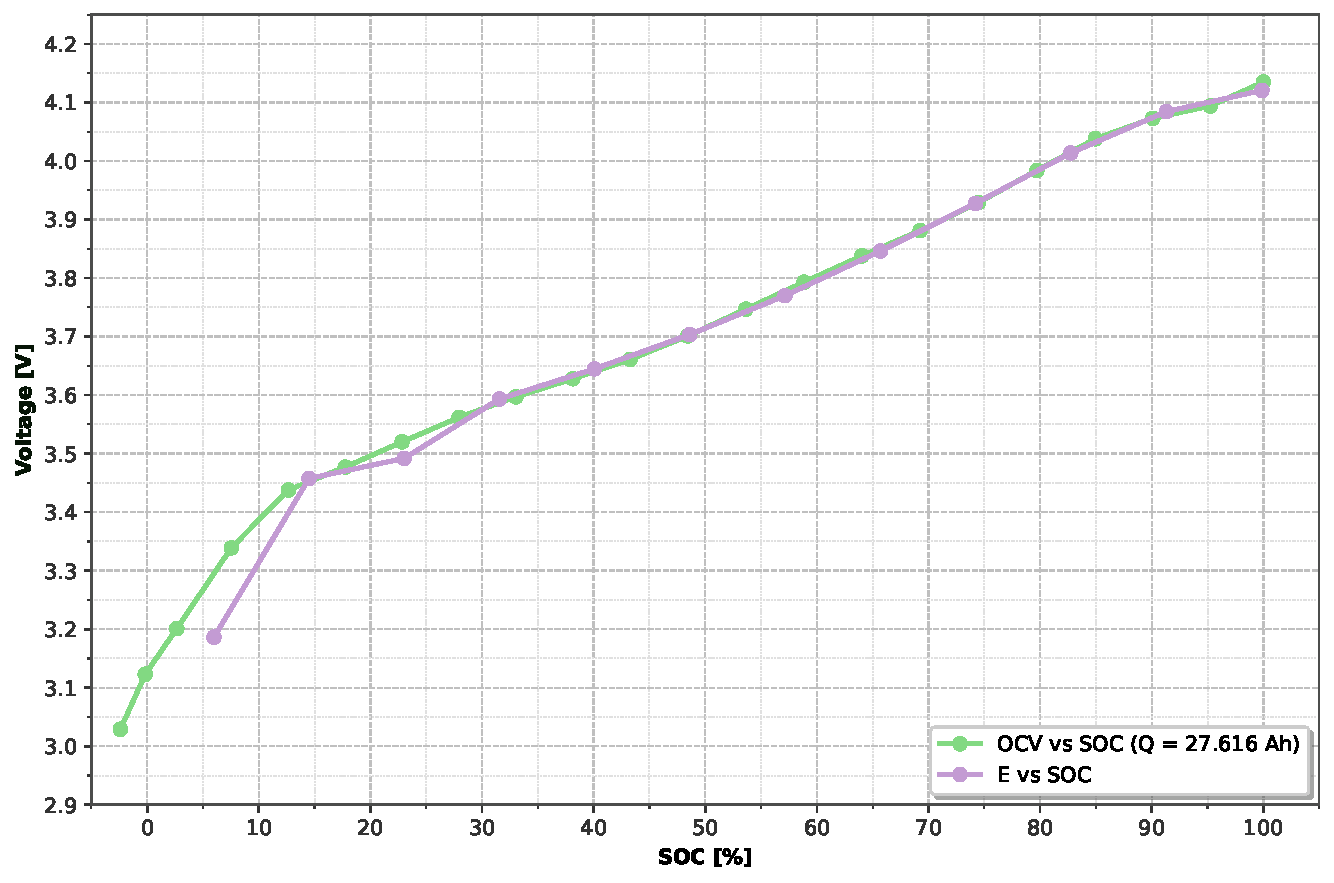
\includegraphics[width = 1\textwidth]{Codigo/Test Baterias/Battery_Graphs_Tests/OCV_and_E_vs_SOC_combined.pdf}
    \caption{OCV vs. SOC curves, obtained through algebraic method (lilac)~\cite{DEVARAKONDA2014} and curve obtained by pulse test (green) 
    in Section~\ref{PulsesTestsResults} of the \acs{NMC} battery}
    \label{ECurveParamResult}
\end{figure}

\section{Extended Kalman Filter}
\subsection{Estimation of SOC with EKF}\label{ResultsSOC}
The \ac{SOC} \ac{EKF} estimator was evaluated under three operating profiles: a charging cycle, a cyclic pulse discharge, and a random step-current discharge. 

\paragraph{Charge Test}
The results of the charge test are shown in Figures~\ref{ChargeEKFSOCResults} and~\ref{EChargeKFSOCErrorResults}. The \ac{EKF} estimate tracks the 
Coulomb counting reference closely throughout the $115\,\text{min}$ charging 
cycle, with the error remaining within the $3\sigma$ bounds for most of the test. 
A small divergence is observed in the final phase of charging known as the constant-voltage stage, reducing the observability of the cell 
state. The \ac{RMSE} between the \ac{EKF} estimate and the Coulomb counting reference was $0.942\%$.

\begin{figure}[H]
    \centering
    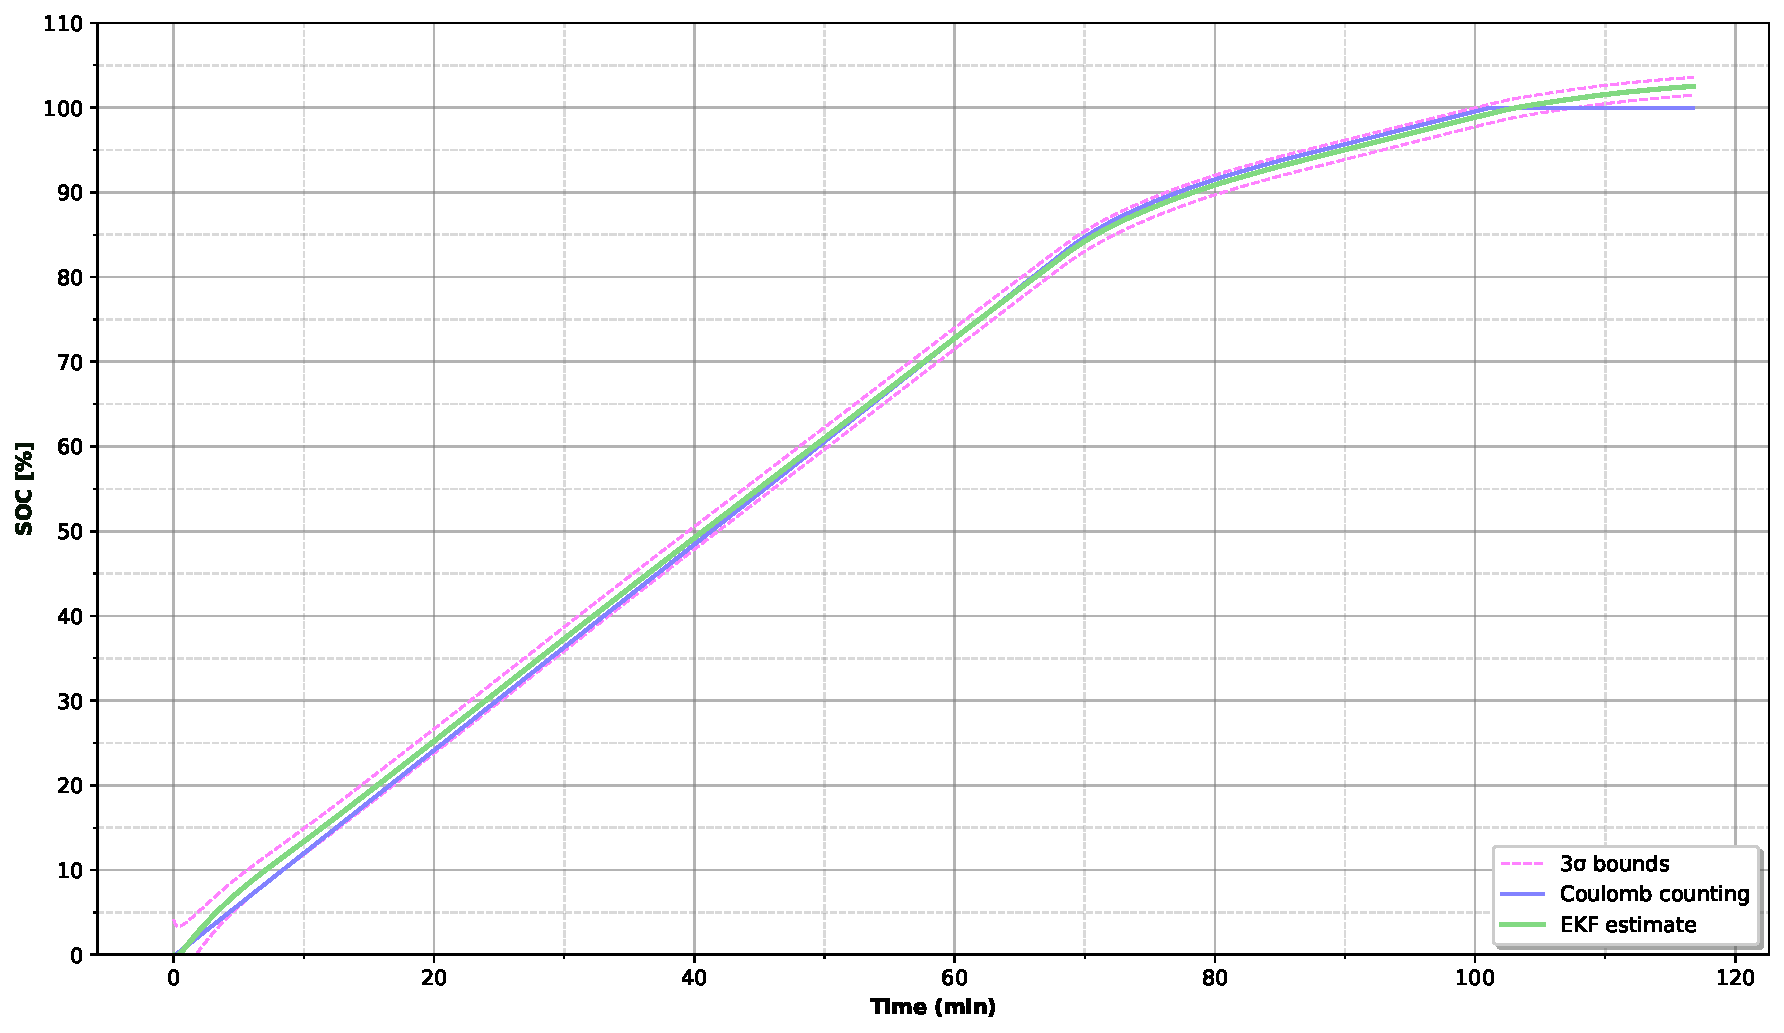
\includegraphics[width = 1\textwidth]{Codigo/Test Baterias/Battery_Graphs_Tests/EKF/soc/EKF_SOC_Charge_Test.pdf}
    \caption{SOC in time comparing Coulomb Counting method (lilac) and EKF estimator (green) during the charging cycle of the \acs{NMC} battery.}
    \label{ChargeEKFSOCResults}
\end{figure}

\begin{figure}[H]
    \centering
    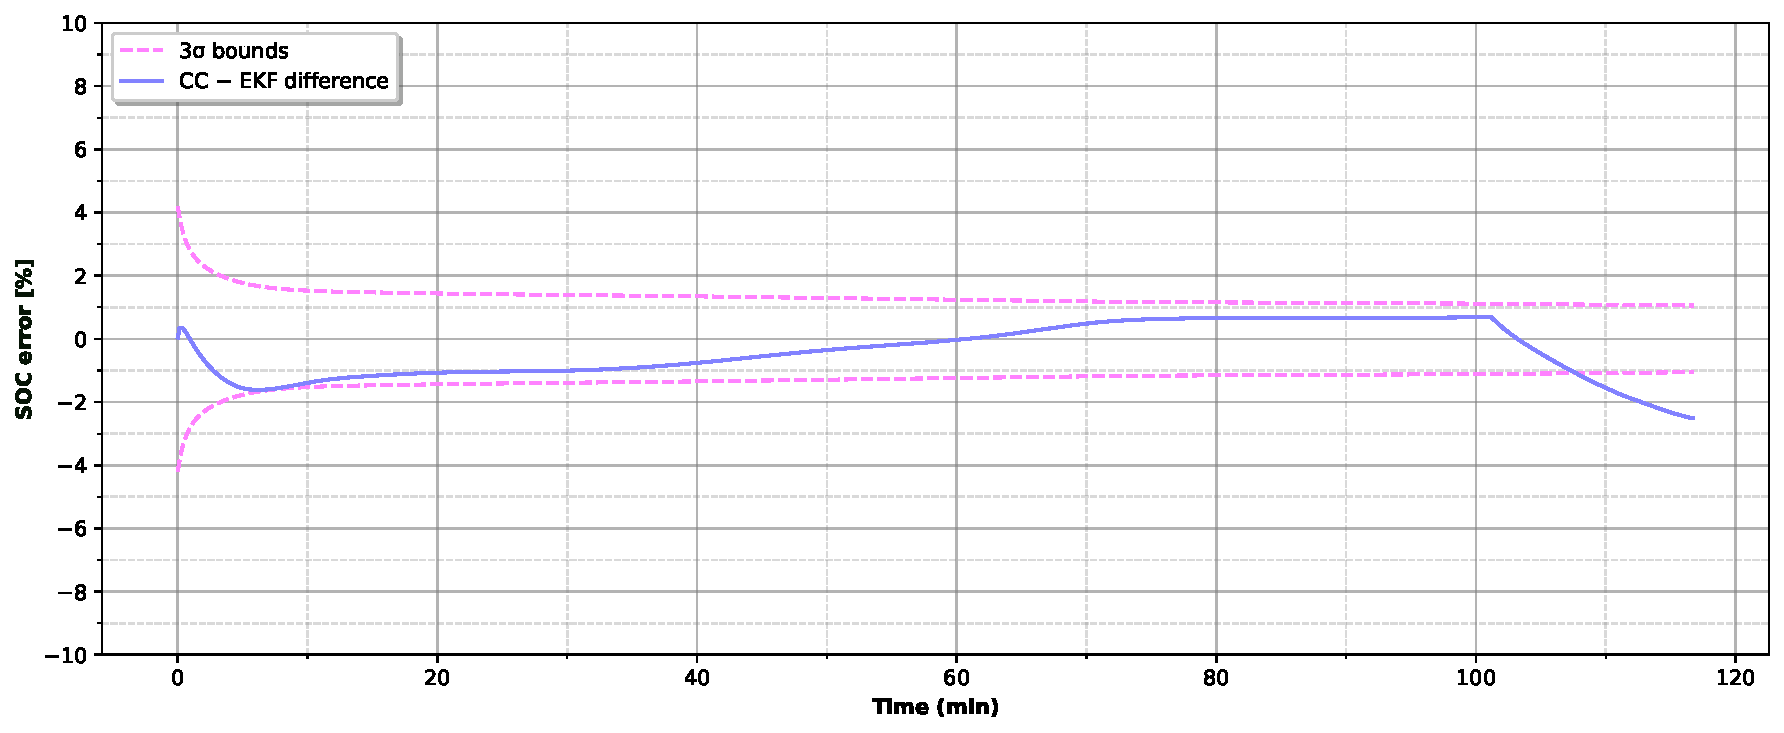
\includegraphics[width = 1\textwidth]{Codigo/Test Baterias/Battery_Graphs_Tests/EKF/soc/EKF_SOC_error_Charge_Test.pdf}
    \caption{Error between CC and EKF SOC estimator during the charging cycle of the \acs{NMC} battery.}
    \label{EChargeKFSOCErrorResults}
\end{figure}

\paragraph{Pulses Test}
During the cyclic pulse discharge test, the current alternated between $10\,A$ and rest at regular intervals. The \ac{EKF} estimate is presented in 
Figures~\ref{PulsesEKFSOCResults} and~\ref{EPulsesKFSOCErrorResults}. 
The filter tracked the step \ac{SOC} decrease over the approximately $300\,\text{min}$ test duration. The estimation error remained 
within the $3\sigma$ bounds throughout, converging to within $\pm 1\%$ of the Coulomb counting reference after the initial transient. The \ac{RMSE} obtained was $1.141\%$.

\begin{figure}[H]
    \centering
    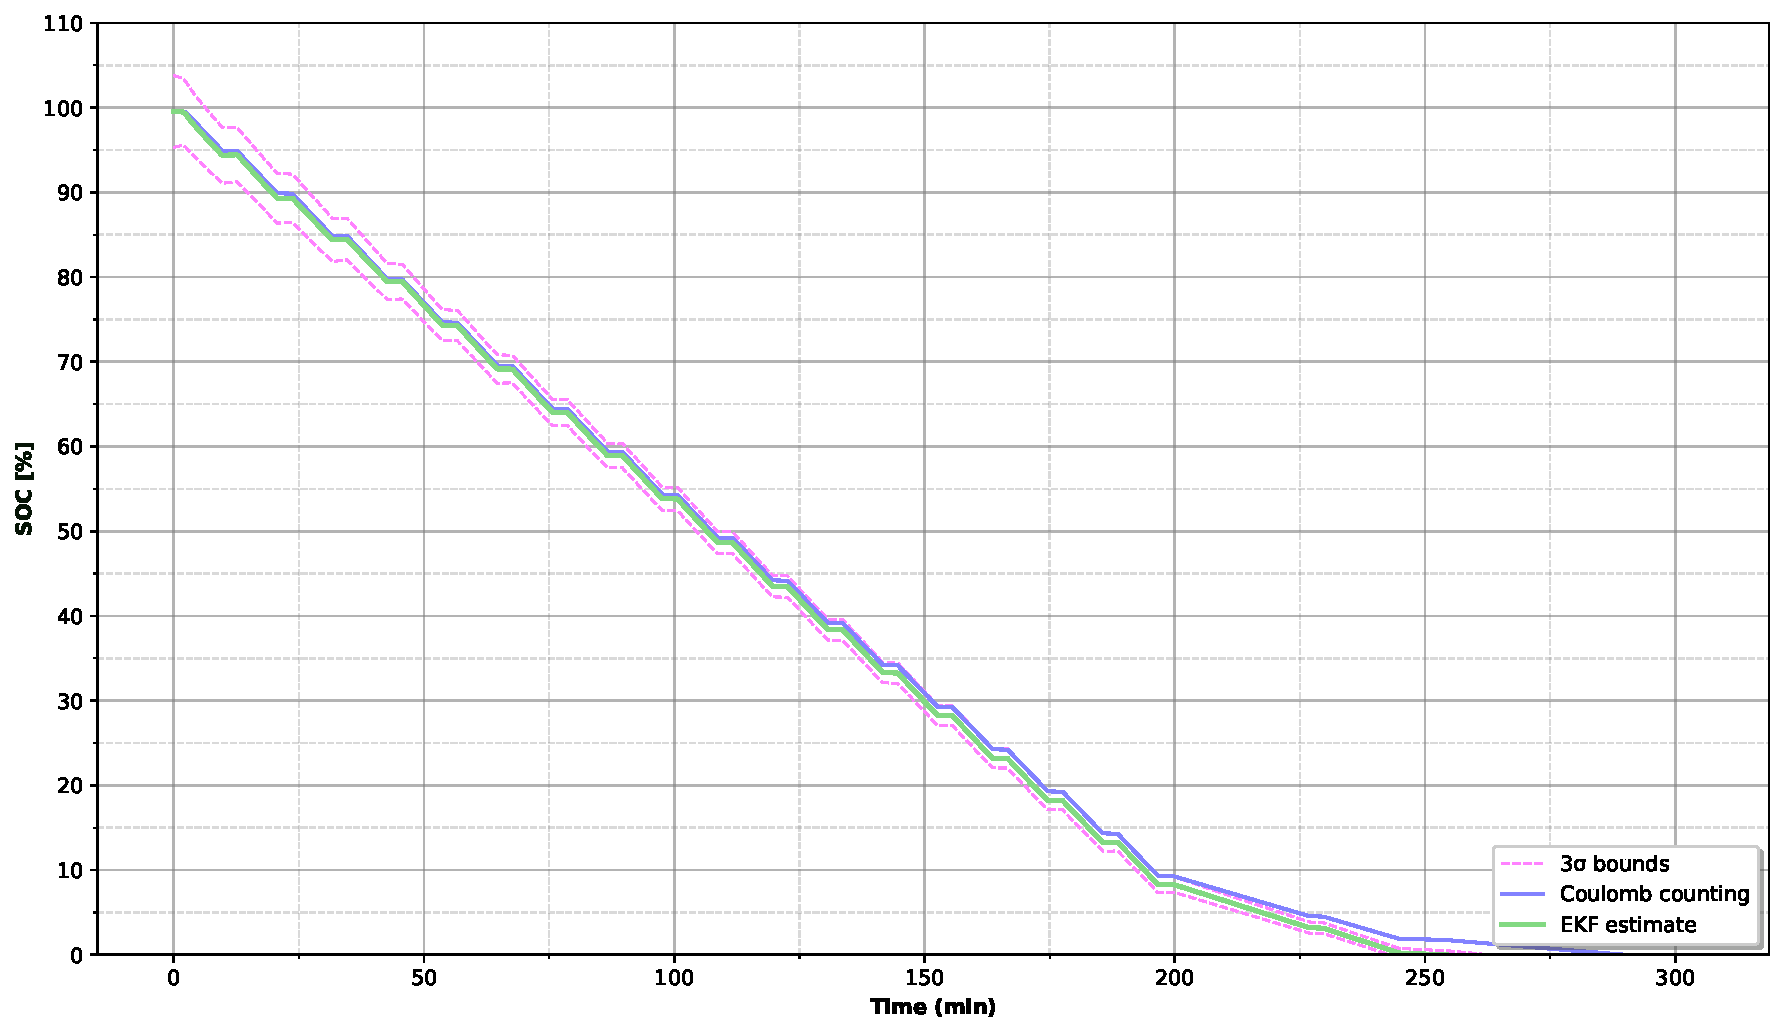
\includegraphics[width = 1\textwidth]{Codigo/Test Baterias/Battery_Graphs_Tests/EKF/soc/EKF_SOC_Pulses_Test.pdf}
    \caption{SOC in time comparing Coulomb Counting method (lilac) and EKF estimator (green) during the pulses cycle of the \acs{NMC} battery.}
    \label{PulsesEKFSOCResults}
\end{figure}

\begin{figure}[H]
    \centering
    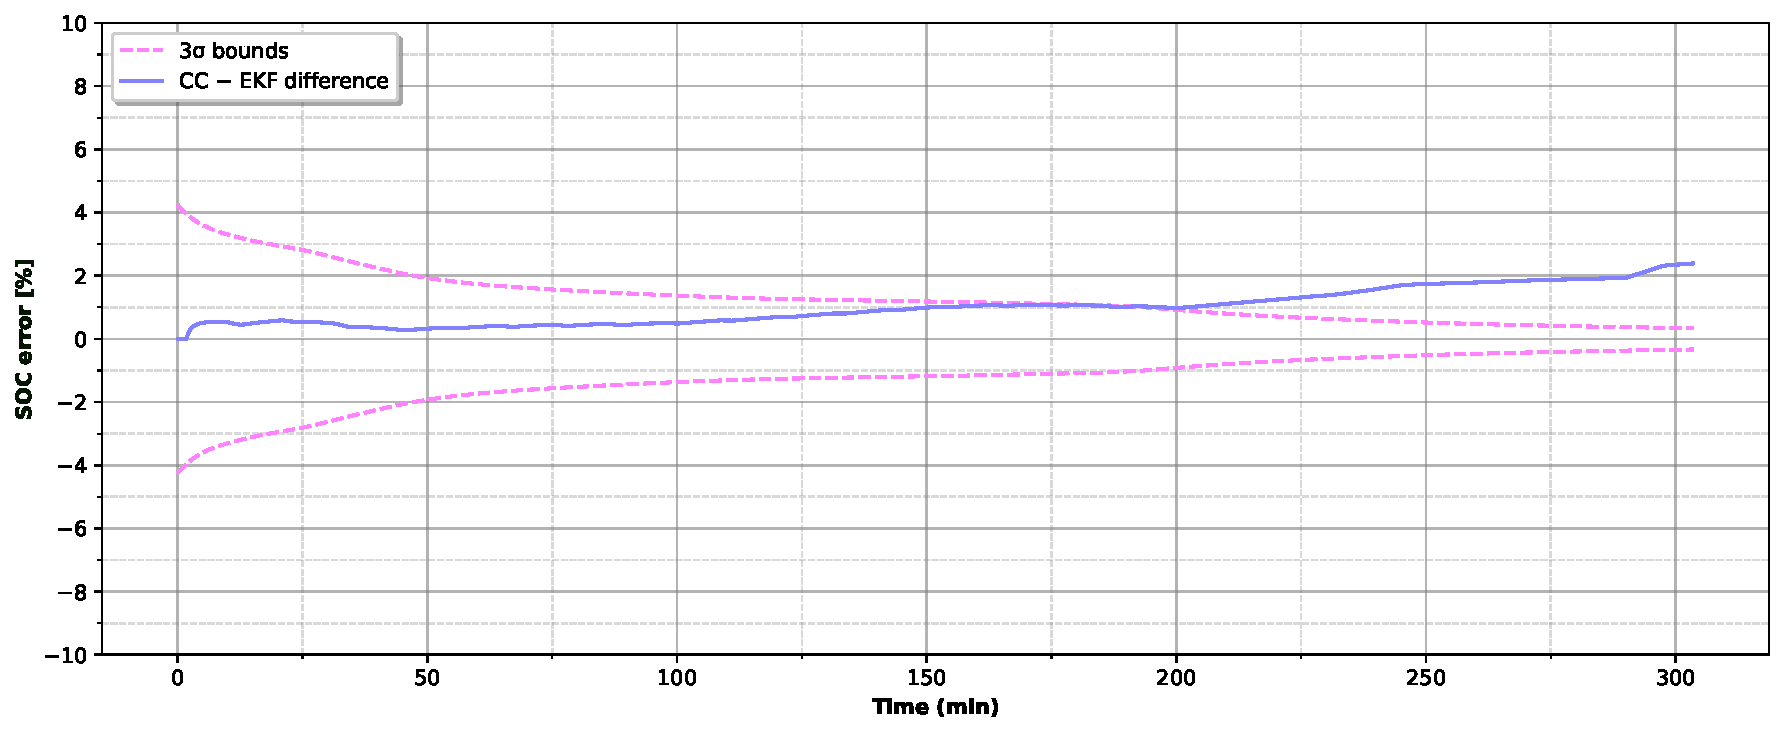
\includegraphics[width = 1\textwidth]{Codigo/Test Baterias/Battery_Graphs_Tests/EKF/soc/EKF_SOC_error_Pulses_Test.pdf}
    \caption{Error between CC and EKF SOC estimator during the pulses cycle of the \acs{NMC} battery.}
    \label{EPulsesKFSOCErrorResults}
\end{figure}

\paragraph{Random Steps Test}
The random step-current profile, alternating between $0\,A$, $10\,A$, and $30\,A$, tested the filter's response to abrupt current changes. Results are presented in 
Figures~\ref{StepsEKFSOCResults} and~\ref{EStepsKFSOCErrorResults}. The \ac{EKF} maintained a similar value to the Coulomb counting reference throughout the 
test. This scenario produced the lowest \ac{RMSE} of the three profiles, at $0.691\%$.

\begin{figure}[H]
    \centering
    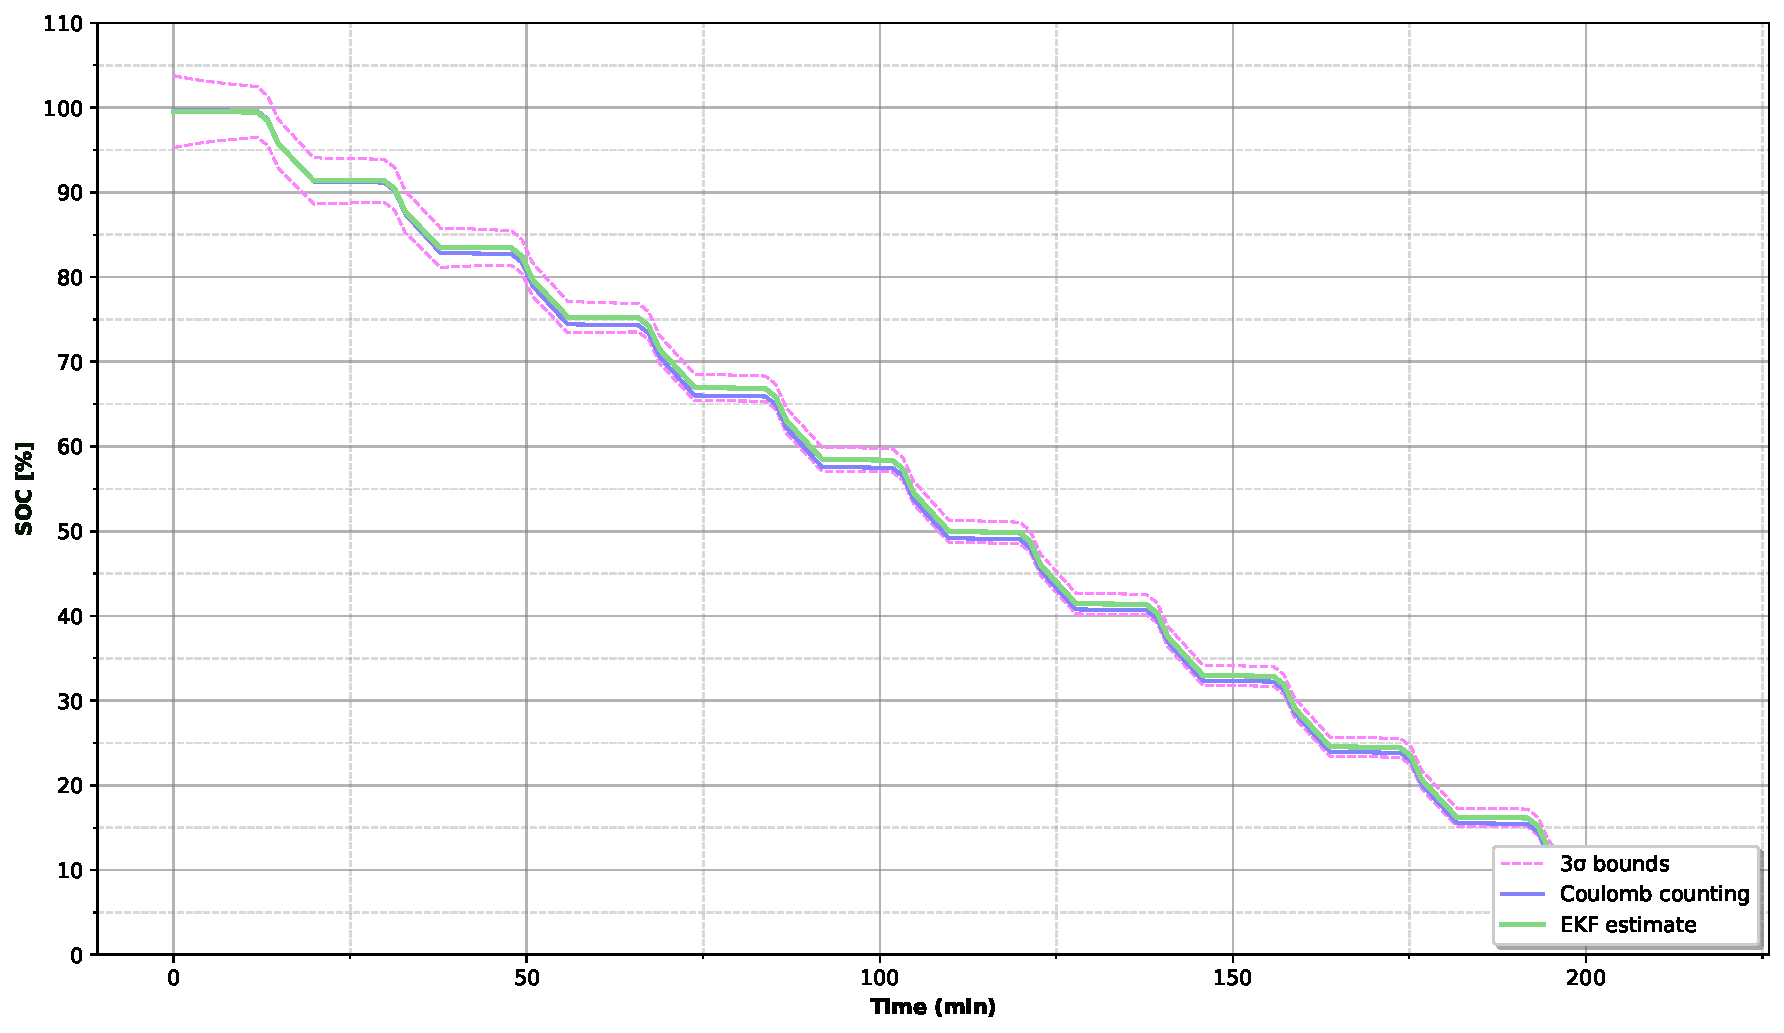
\includegraphics[width = 1\textwidth]{Codigo/Test Baterias/Battery_Graphs_Tests/EKF/soc/EKF_SOC_Steps_Test.pdf}
    \caption{SOC in time comparing Coulomb Counting method (lilac) and EKF estimator (green) during the random steps cycle of the \acs{NMC} battery.}
    \label{StepsEKFSOCResults}
\end{figure}

\begin{figure}[H]
    \centering
    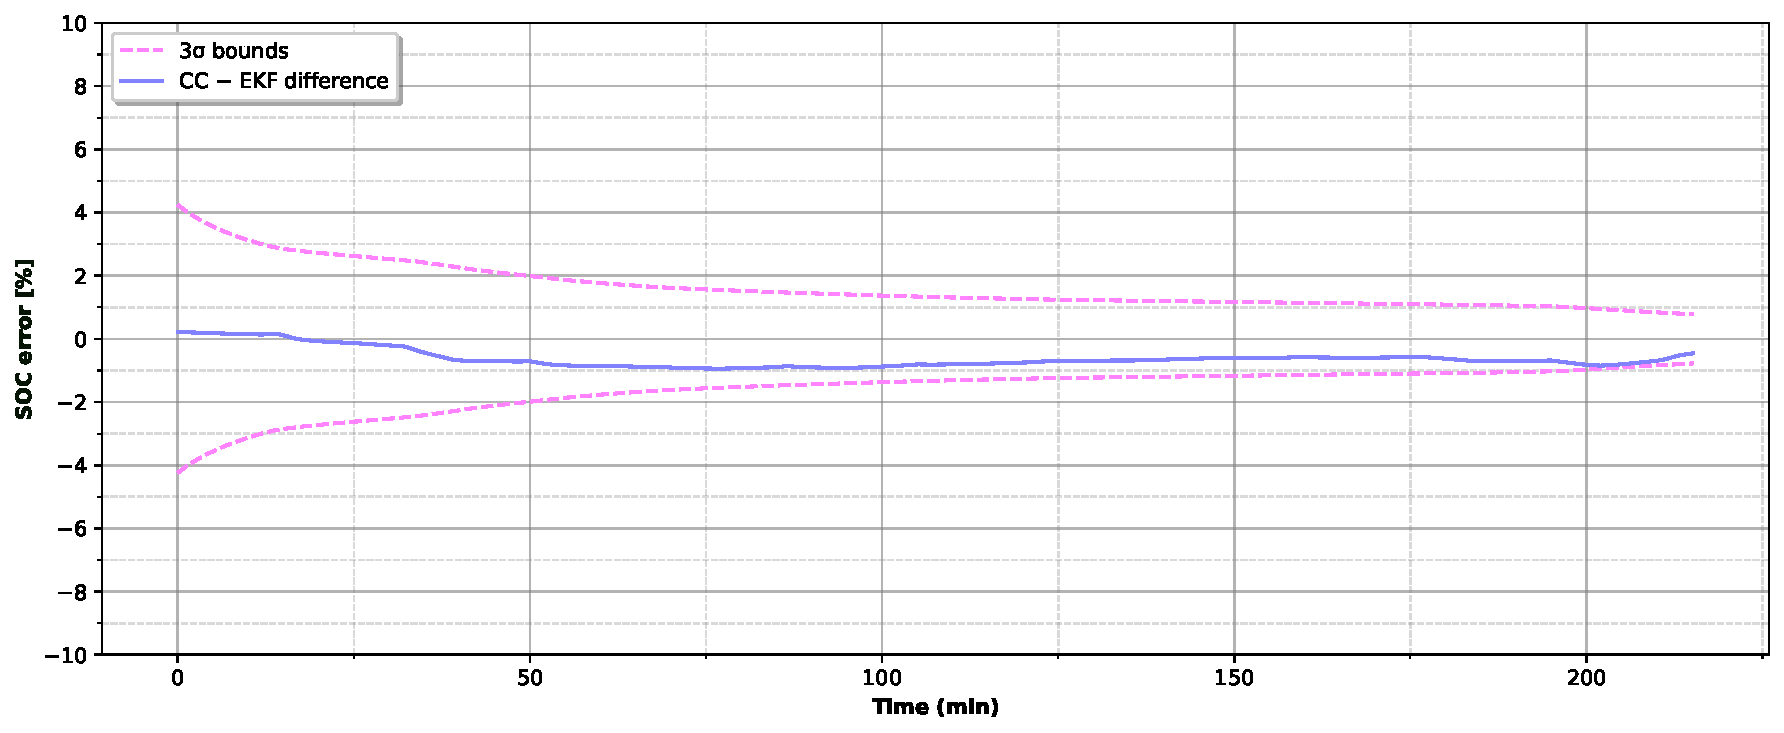
\includegraphics[width = 1\textwidth]{Codigo/Test Baterias/Battery_Graphs_Tests/EKF/soc/EKF_SOC_error_Steps_Test.pdf}
    \caption{Error between CC and EKF SOC estimator during the random steps cycle of the \acs{NMC} battery.}
    \label{EStepsKFSOCErrorResults}
\end{figure}

\subsection{Estimation of \acs{SOC} and \acs{SOH} with Dual \acs{EKF}}\label{ResultsSOC&SOH}
The dual \ac{EKF} was applied to the same three test profiles, simultaneously estimating the \ac{SOC} and the \ac{SOH}, the last state consisting in parameters $R_0$ and $Q$. 
Both parameters were initialised at the values established during cell characterisation. 
A warm-up period of 500 samples was used, during which the parameter filter accumulated the sensitivity information required for reliable estimation before 
beginning to update $R_0$ and $Q$.

\paragraph{Charge Test}
The estimated capacity $Q$ and series resistance $R_0$ are presented in Figures~\ref{Charge_Q_EKFSOCSOHResults} and~\ref{Charge_R0_EKFSOCSOHResults}, 
respectively. At the end of the test, the capacity estimate had converged to $28.44\,\text{Ah}$, $3\sigma = \pm 0.58\,\text{Ah}$
and the resistance estimate to $R_0 = 2.246\,\text{m}\Omega$, $3\sigma = \pm 0.462\,\text{m}\Omega$.

\begin{figure}[H]
    \centering
    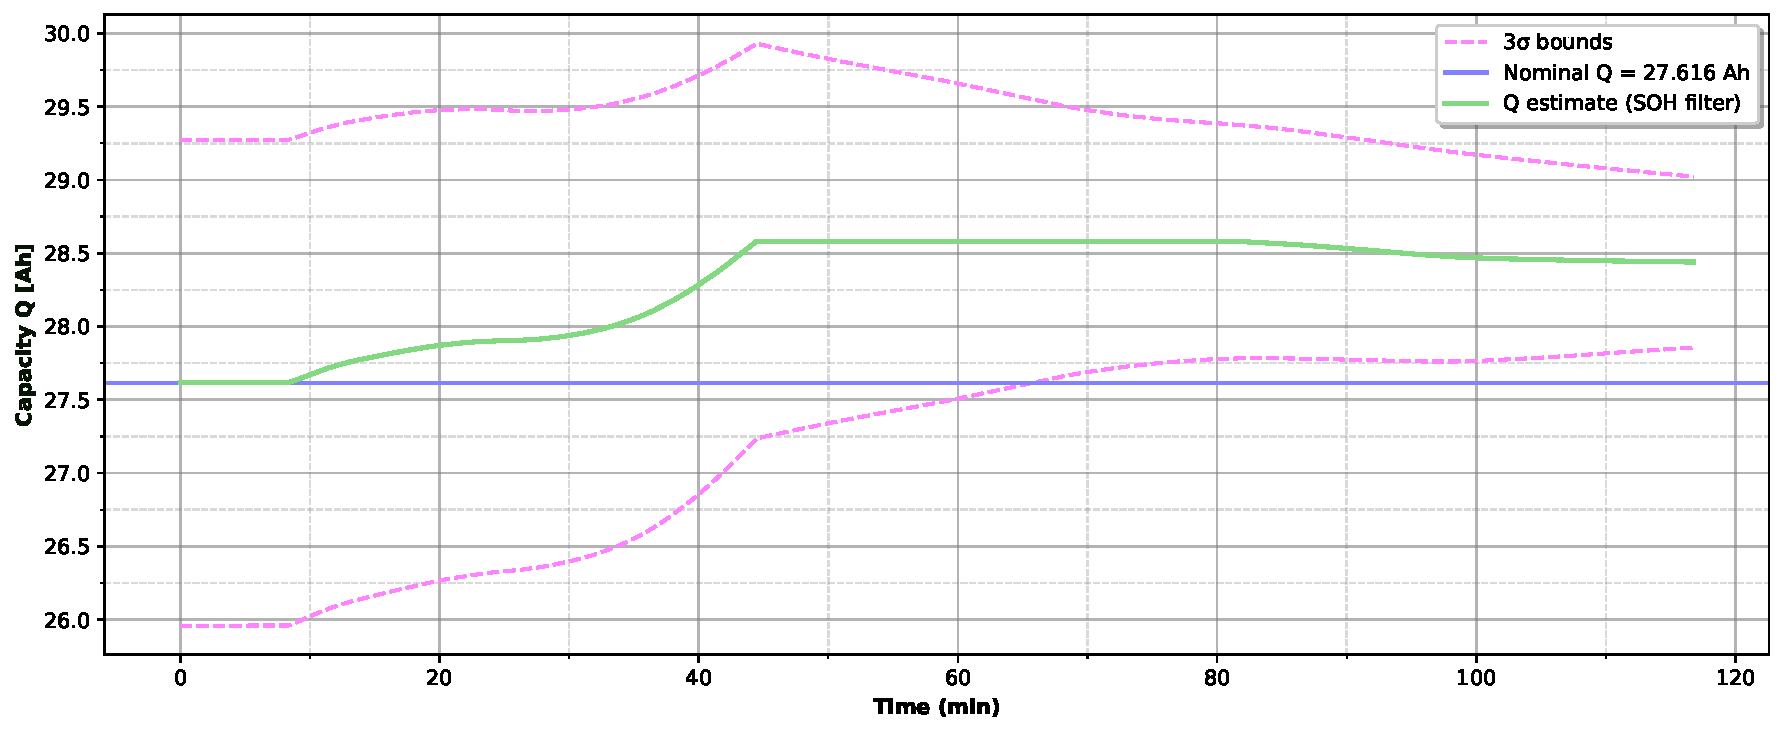
\includegraphics[width = 1\textwidth]{Codigo/Test Baterias/Battery_Graphs_Tests/EKF/dual/EKF_Q_Charge_Test.pdf}
    \caption{Capacity evolution during the \acs{CC-CV} charging cycle of the \acs{NMC} 
    battery (constant-current phase at $20\,\text{A}$ up to approximately 
    $70\,\text{min}$, followed by the constant-voltage phase until the current dropped 
    below $2.009\,\text{A}$), sampled at $\Delta t = 1\,\text{s}$. 
    Estimated capacity (green) and nominal capacity (lilac).}
    \label{Charge_Q_EKFSOCSOHResults}
\end{figure}

\begin{figure}[H]
    \centering
    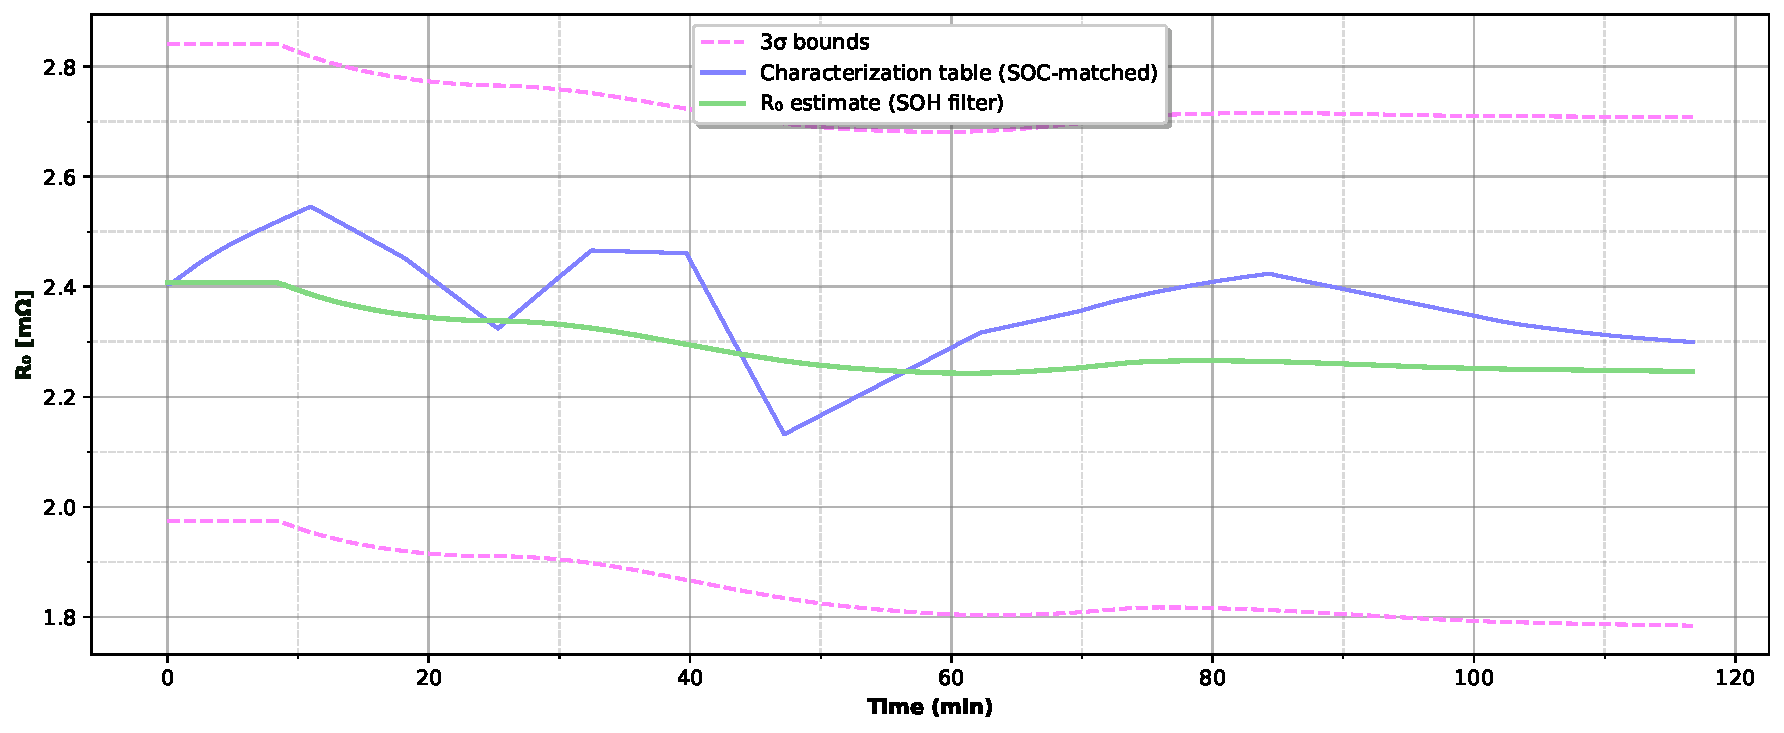
\includegraphics[width = 1\textwidth]{Codigo/Test Baterias/Battery_Graphs_Tests/EKF/dual/EKF_R0_Charge_Test.pdf}
    \caption{Resistor $R_0$ evolution during the \acs{CC-CV} charging cycle of the 
    \acs{NMC} battery (constant-current phase at $20\,\text{A}$ up to approximately 
    $70\,\text{min}$, followed by the constant-voltage phase), sampled at 
    $\Delta t = 1\,\text{s}$. Estimated resistor (green) and characterised resistor (lilac).}
    \label{Charge_R0_EKFSOCSOHResults}
\end{figure}

The \ac{SOC} estimate for the charge test is shown in Figure~\ref{ChargeEKFSOCSOHResults}, with the corresponding error in 
Figure~\ref{EChargeKFSOCSOHErrorResults}. The \ac{RMSE} versus Coulomb counting 
was $1.390\%$, higher than the \ac{SOC}-only estimator result, which is expected since the dual filter simultaneously adapts the capacity estimate. 

\begin{figure}[H]
    \centering
    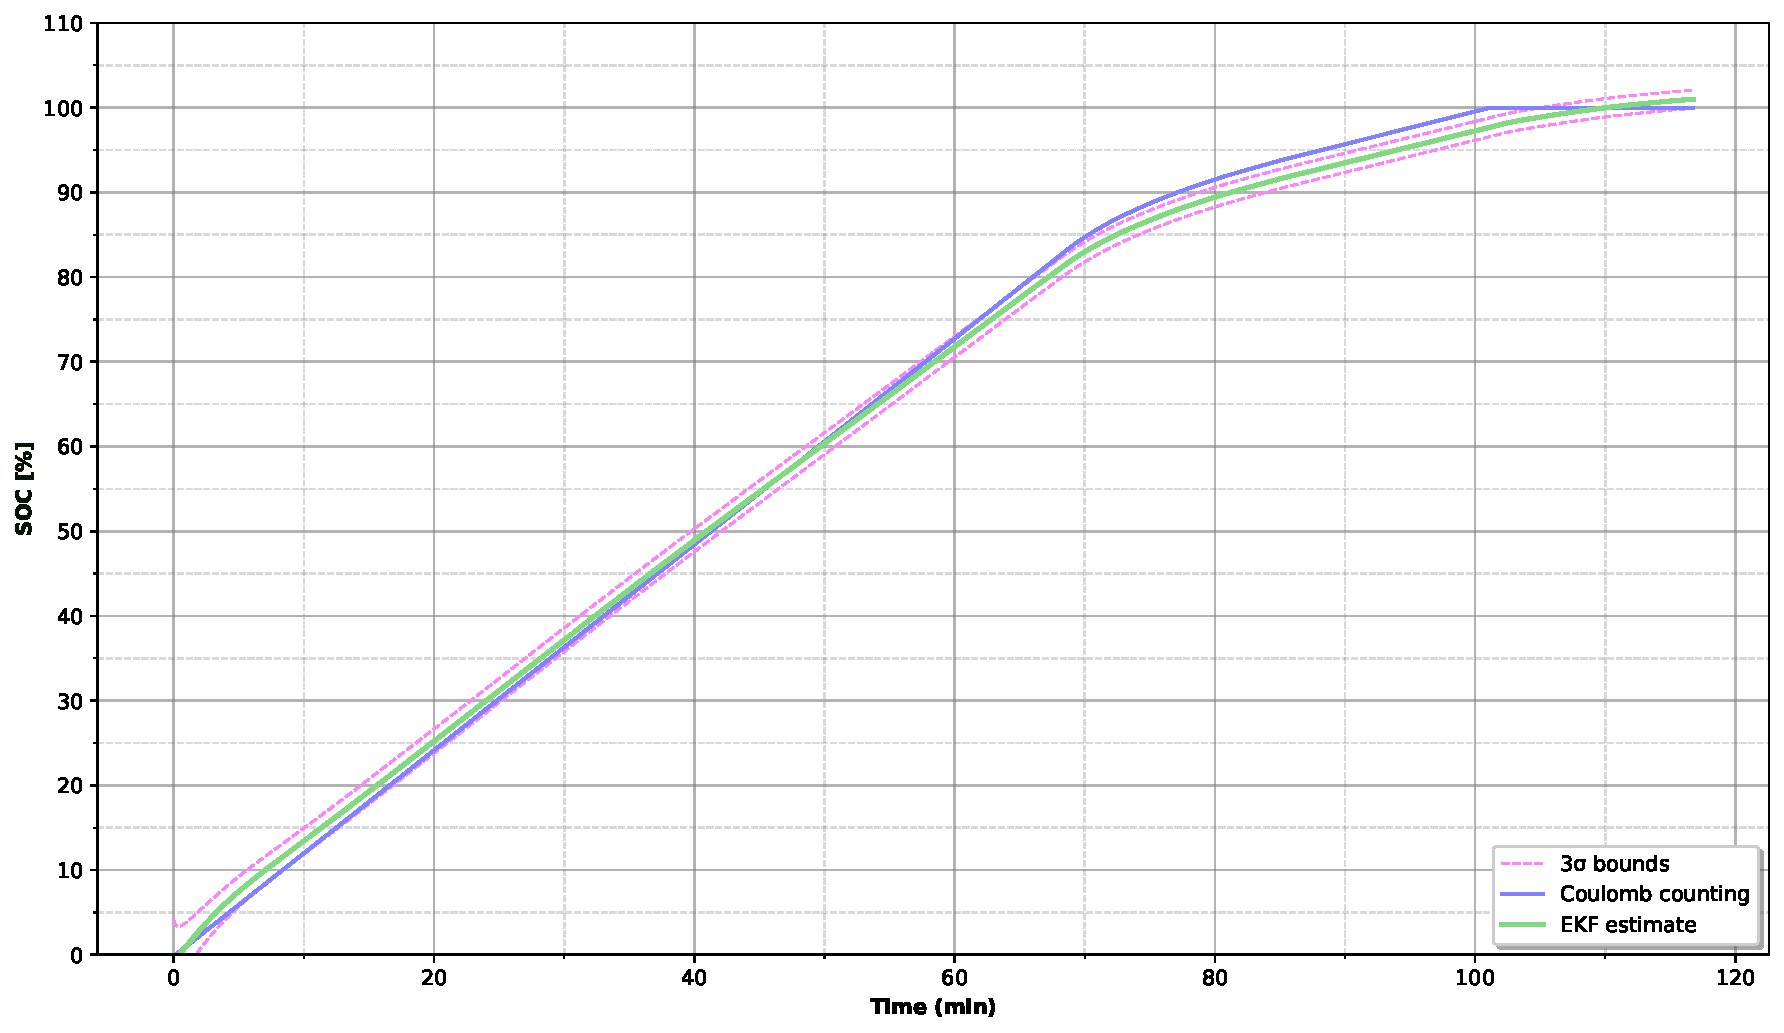
\includegraphics[width = 1\textwidth]{Codigo/Test Baterias/Battery_Graphs_Tests/EKF/dual/EKF_SOC_Charge_Test.pdf}
    \caption{SOC in time comparing Coulomb Counting method (lilac) and SOC \& SOH EKF estimator (green) during the charging cycle of the \acs{NMC} battery.}
    \label{ChargeEKFSOCSOHResults}
\end{figure}

\begin{figure}[H]
    \centering
    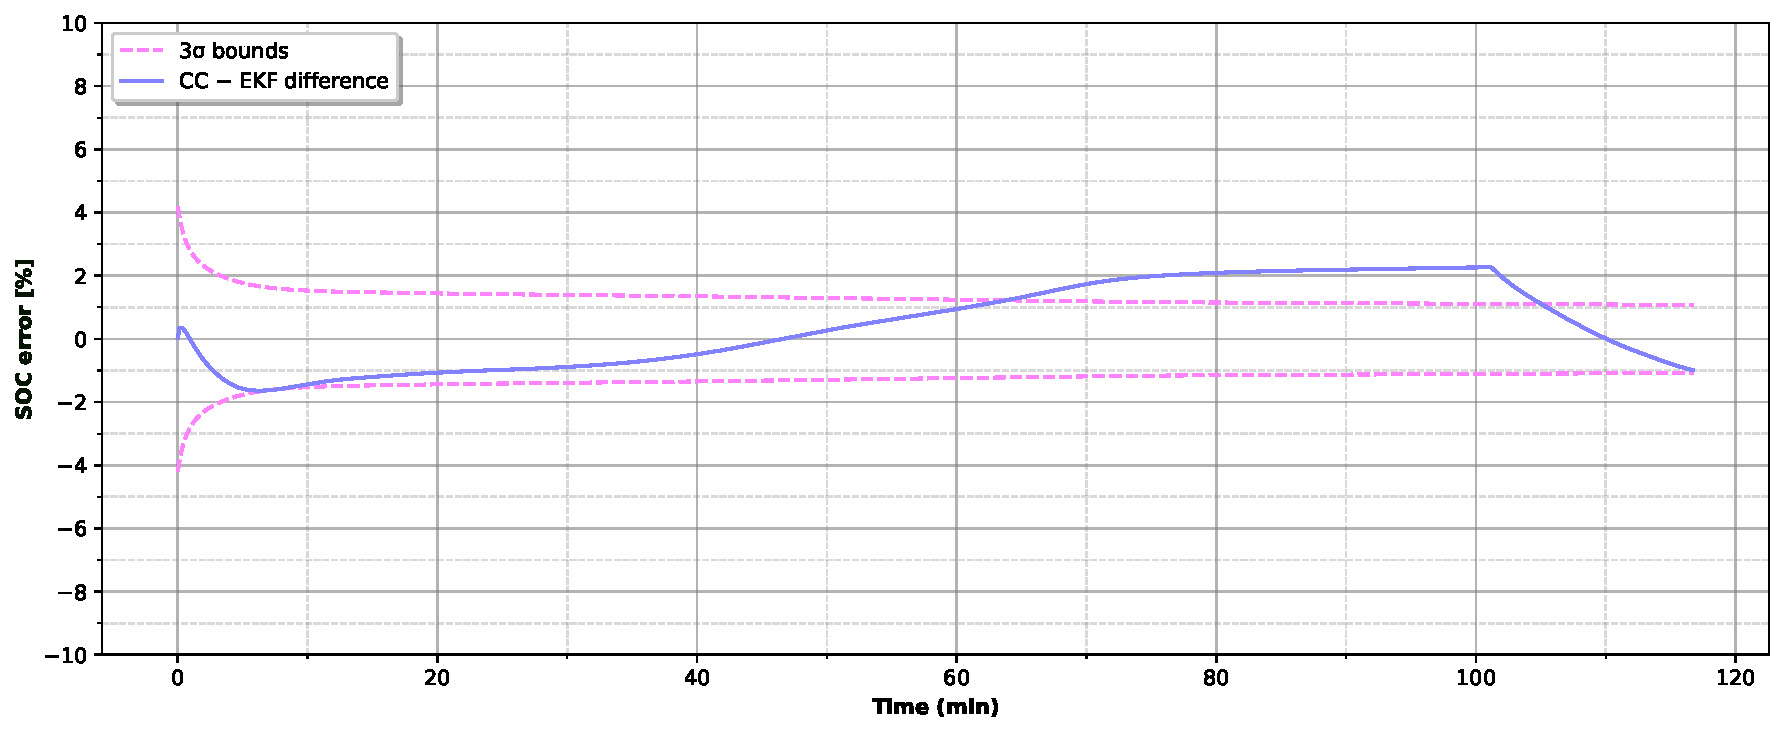
\includegraphics[width = 1\textwidth]{Codigo/Test Baterias/Battery_Graphs_Tests/EKF/dual/EKF_SOC_error_Charge_Test.pdf}
    \caption{Error between CC and dual EKF SOC estimator during the charging cycle of the \acs{NMC} battery.}
    \label{EChargeKFSOCSOHErrorResults}
\end{figure}

\paragraph{Pulses Test}
The capacity estimate converged to $27.67\,\text{Ah}$, $3\sigma = \pm 0.10\,\text{Ah}$, 
closely matching the characterised value. The series resistance converged to $2.134\,\text{m}\Omega$, $3\sigma = \pm 0.540\,\text{m}\Omega$. 
The estimated $R_0$ remained within the characterisation table range throughout, as shown in Figure~\ref{Pulses_R0_EKFSOCSOHResults}.

\begin{figure}[H]
    \centering
    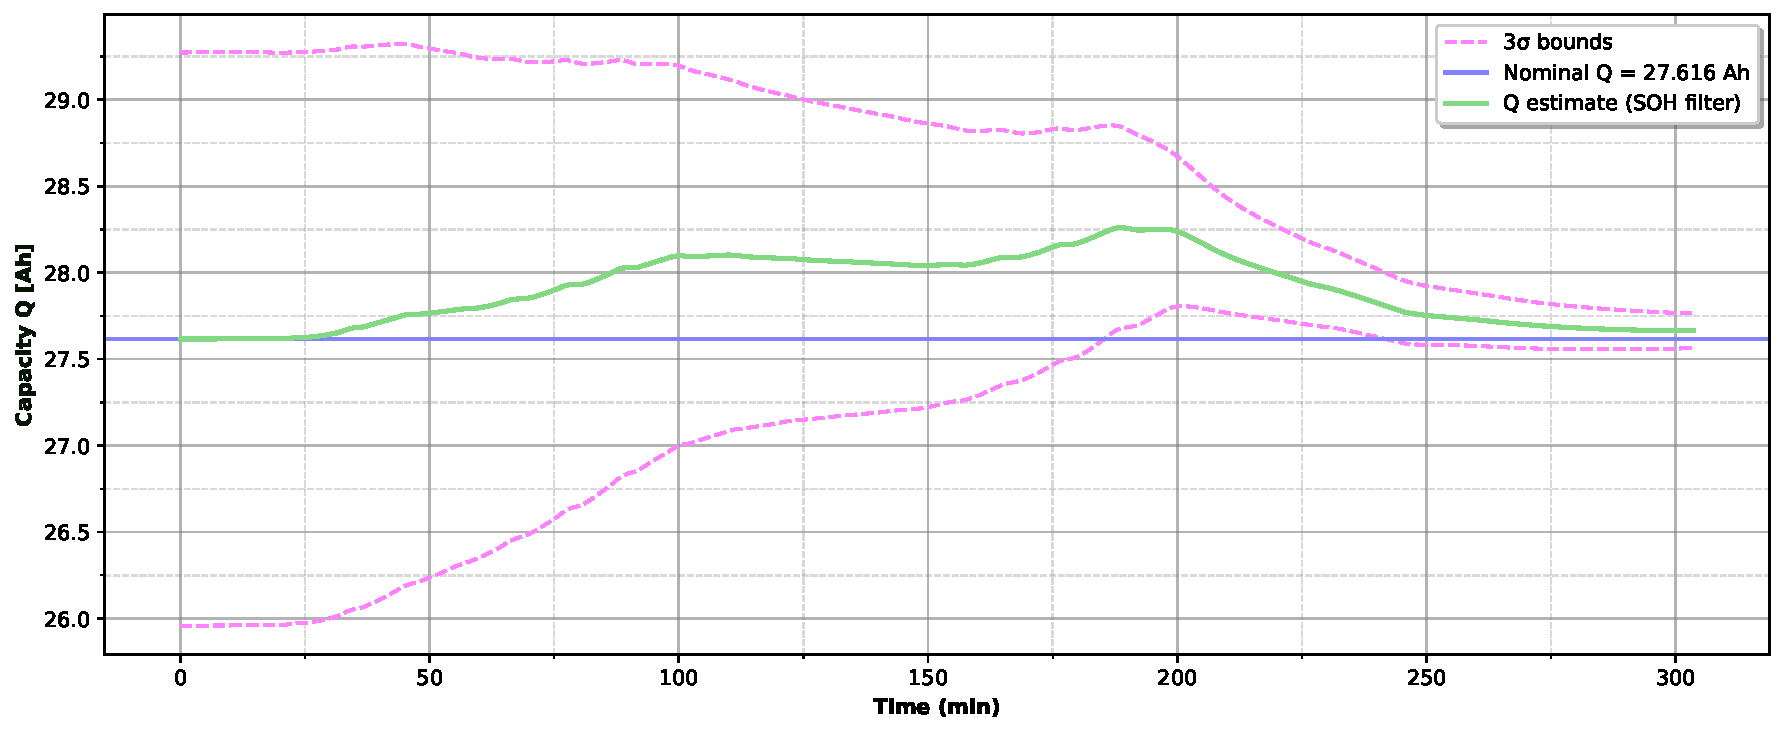
\includegraphics[width = 1\textwidth]{Codigo/Test Baterias/Battery_Graphs_Tests/EKF/dual/EKF_Q_Pulses_Test.pdf}
    \caption{Capacity evolution during the cyclic pulse discharge of the \acs{NMC} 
    battery ($10\,\text{A}$ pulses of $10\,\text{min}$ separated by $3\,\text{min}$ 
    rest periods, until full discharge), sampled at $\Delta t = 1\,\text{s}$. Estimated capacity (green) and nominal capacity (lilac).}
    \label{Pulses_Q_EKFSOCSOHResults}
\end{figure}

\begin{figure}[H]
    \centering
    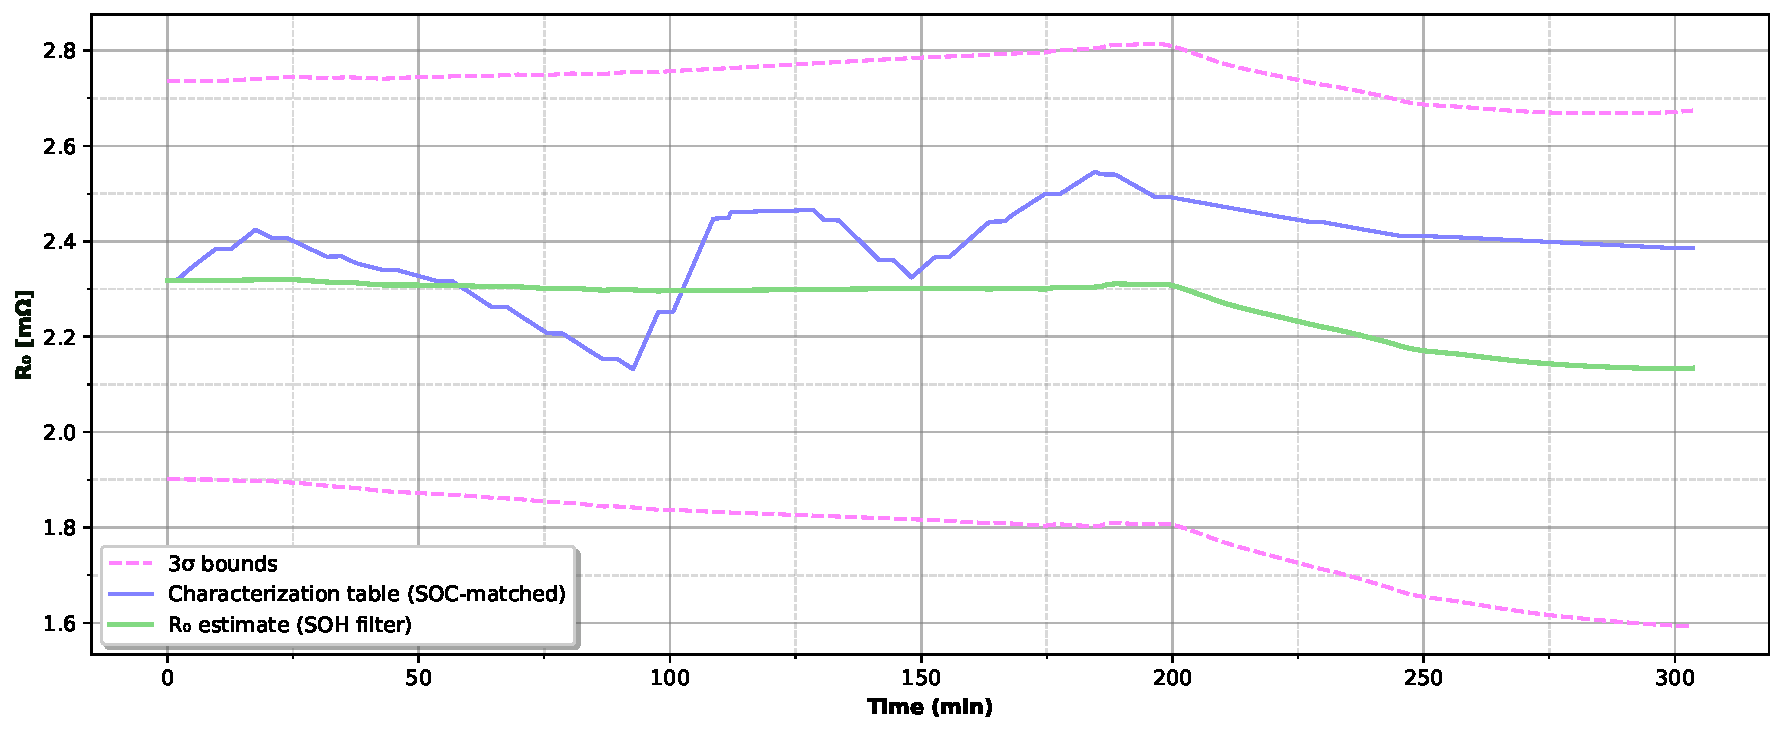
\includegraphics[width = 1\textwidth]{Codigo/Test Baterias/Battery_Graphs_Tests/EKF/dual/EKF_R0_Pulses_Test.pdf}
    \caption{Resistor evolution during the cyclic pulse discharge of the \acs{NMC} 
    battery ($10\,\text{A}$ pulses of $10\,\text{min}$ separated by $3\,\text{min}$ 
    rest periods, until full discharge), sampled at $\Delta t = 1\,\text{s}$. Estimated resistor (green) and characterised resistor (lilac).}
    \label{Pulses_R0_EKFSOCSOHResults}
\end{figure}

Results for the cyclic pulse discharge are shown in Figures~\ref{Pulses_Q_EKFSOCSOHResults}--\ref{EPulsesKFSOCSOHErrorResults}. 
The \ac{SOC} \ac{RMSE} was $0.943\%$.

\begin{figure}[H]
    \centering
    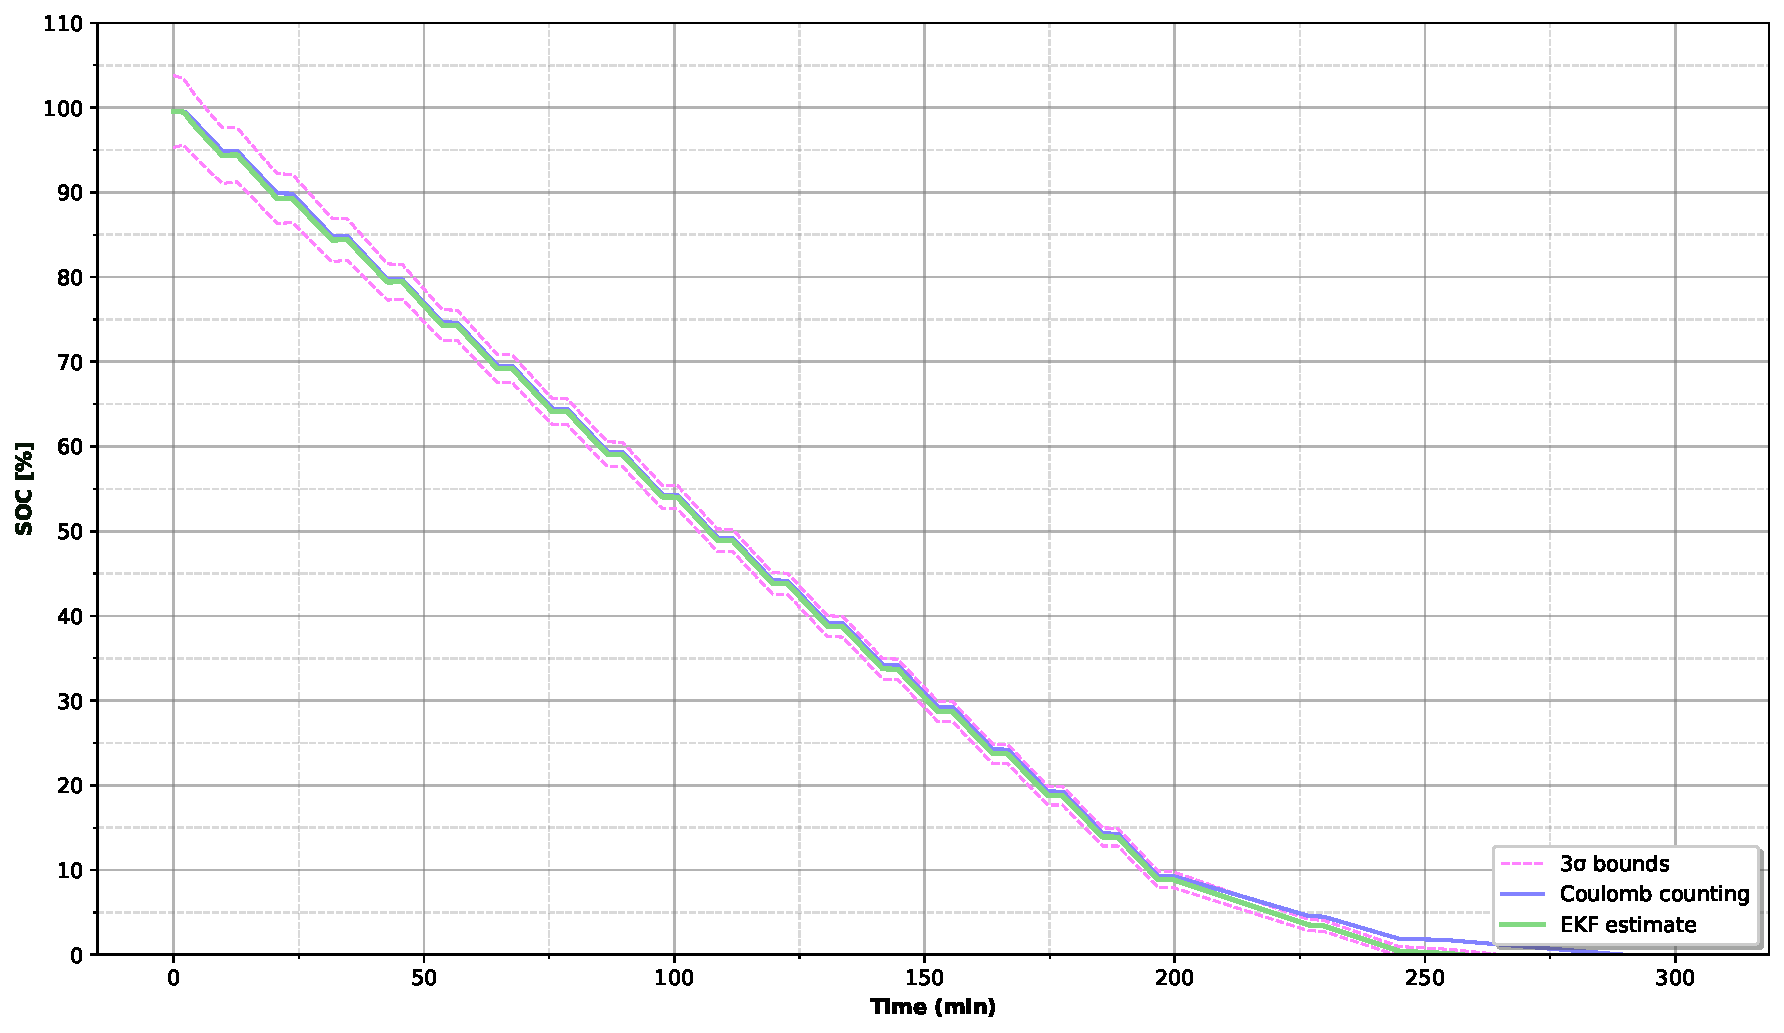
\includegraphics[width = 1\textwidth]{Codigo/Test Baterias/Battery_Graphs_Tests/EKF/dual/EKF_SOC_Pulses_Test.pdf}
    \caption{SOC in time comparing Coulomb Counting method (lilac) and SOC \& SOH EKF estimator (green) during the pulses cycle of the \acs{NMC} battery.}
    \label{PulsesEKFSOCSOHResults}
\end{figure}

\begin{figure}[H]
    \centering
    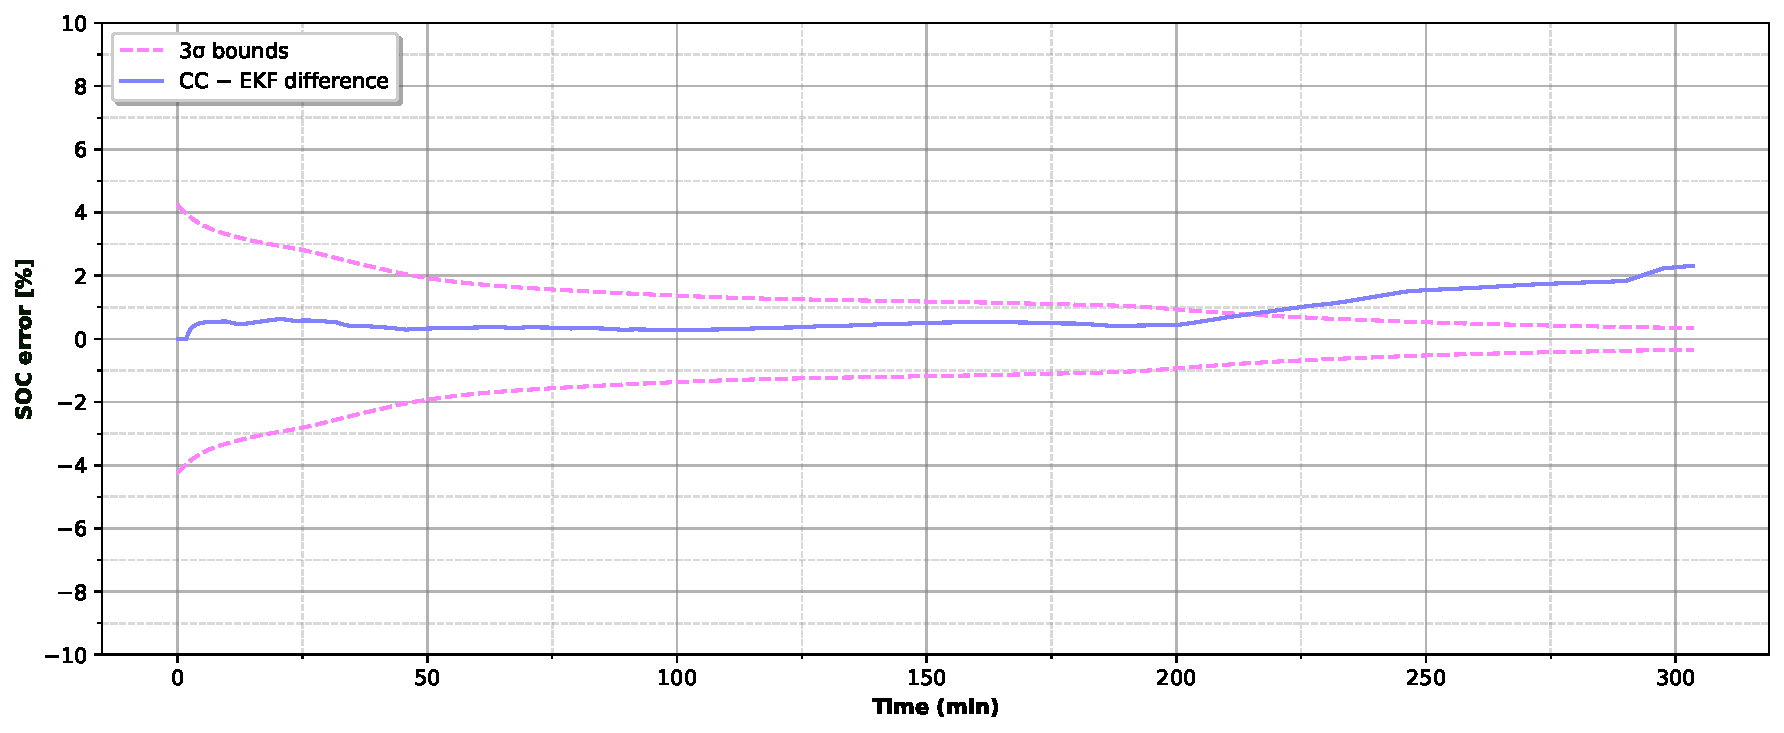
\includegraphics[width = 1\textwidth]{Codigo/Test Baterias/Battery_Graphs_Tests/EKF/dual/EKF_SOC_error_Pulses_Test.pdf}
    \caption{Error between CC and dual EKF SOC estimator during the pulses cycle of the \acs{NMC} battery.}
    \label{EPulsesKFSOCSOHErrorResults}
\end{figure}

\paragraph{Random Steps Test}
The final capacity estimate was $27.92\,\text{Ah}$, $3\sigma = \pm 0.32\,\text{Ah}$ and the 
resistance estimate $2.132\,\text{m}\Omega$, $3\sigma = \pm 0.468\,\text{m}\Omega$. The higher current values of 
this profile resulted in faster initial convergence of $R_0$ compared to the constant-current tests, as visible in Figure~\ref{Steps_R0_EKFSOCSOHResults}.

\begin{figure}[H]
    \centering
    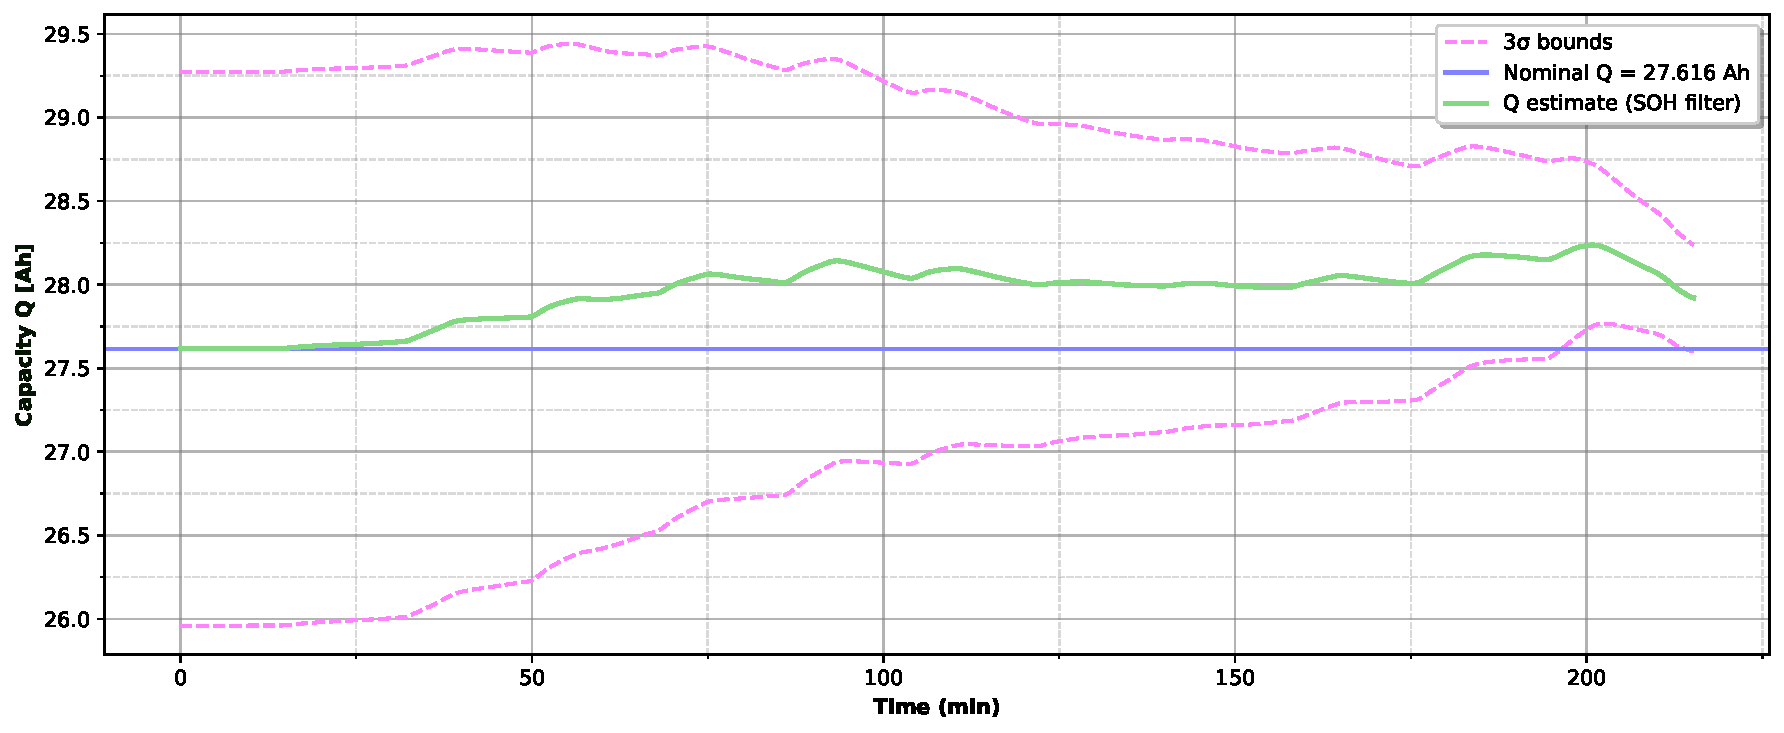
\includegraphics[width = 1\textwidth]{Codigo/Test Baterias/Battery_Graphs_Tests/EKF/dual/EKF_Q_Steps_Test.pdf}
    \caption{apacity evolution during the random step-current discharge of the 
    \acs{NMC} battery (steps between $0\,\text{A}$, $10\,\text{A}$, and $30\,\text{A}$), 
    sampled at $\Delta t = 1\,\text{s}$. Estimated capacity (green) and nominal capacity (lilac).}
    \label{Steps_Q_EKFSOCSOHResults}
\end{figure}

\begin{figure}[H]
    \centering
    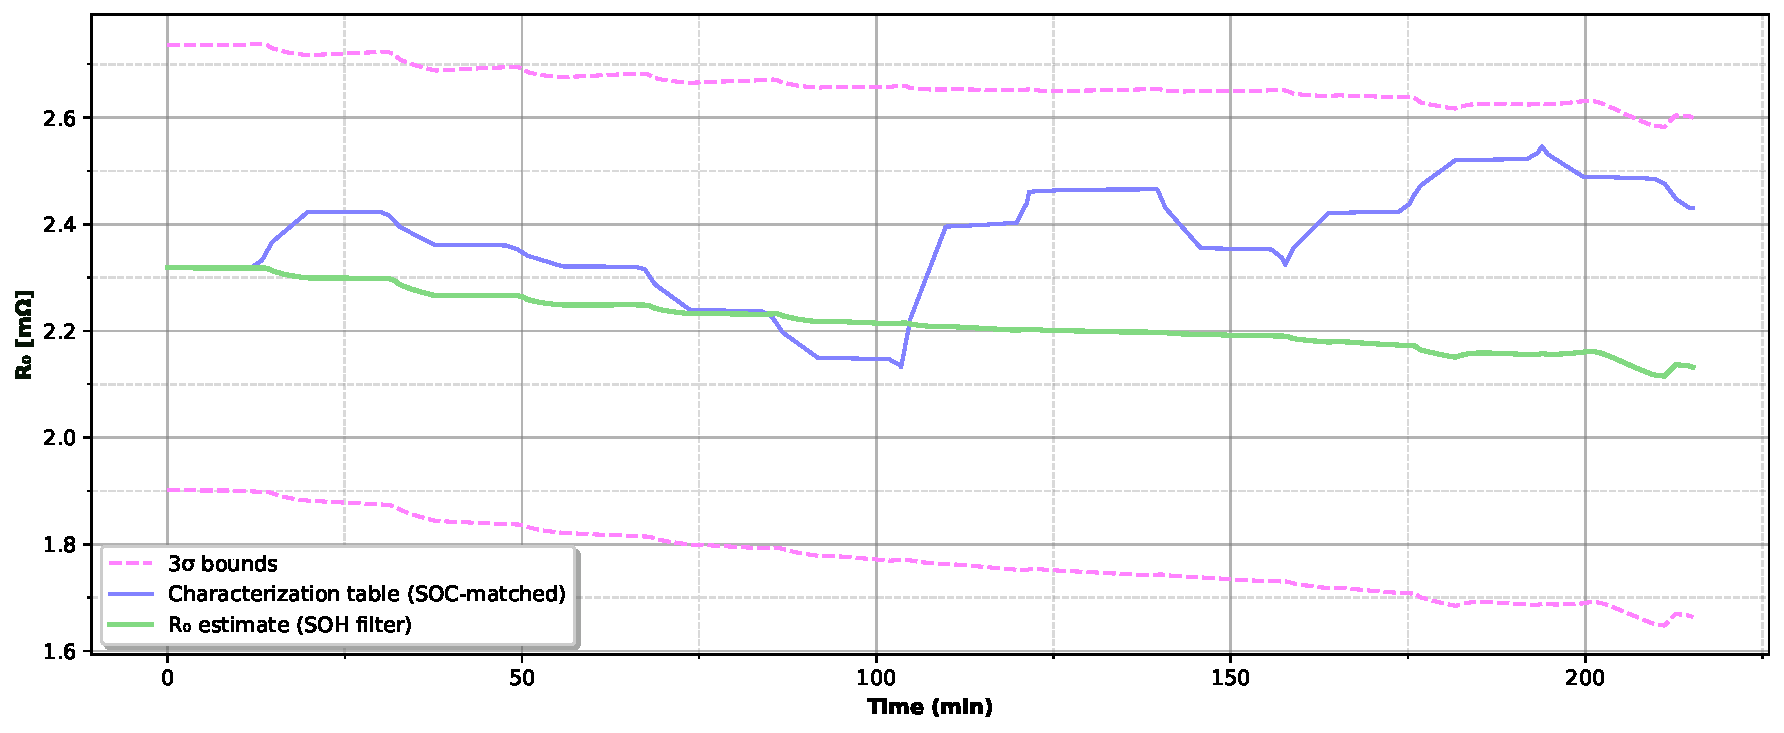
\includegraphics[width = 1\textwidth]{Codigo/Test Baterias/Battery_Graphs_Tests/EKF/dual/EKF_R0_Steps_Test.pdf}
    \caption{Resistor $R_0$ evolution during the random step-current discharge of the 
    \acs{NMC} battery (steps between $0\,\text{A}$, $10\,\text{A}$, and $30\,\text{A}$), 
    sampled at $\Delta t = 1\,\text{s}$. Estimated resistor (green) and characterised resistor (lilac).}
    \label{Steps_R0_EKFSOCSOHResults}
\end{figure}


\begin{figure}[H]
    \centering
    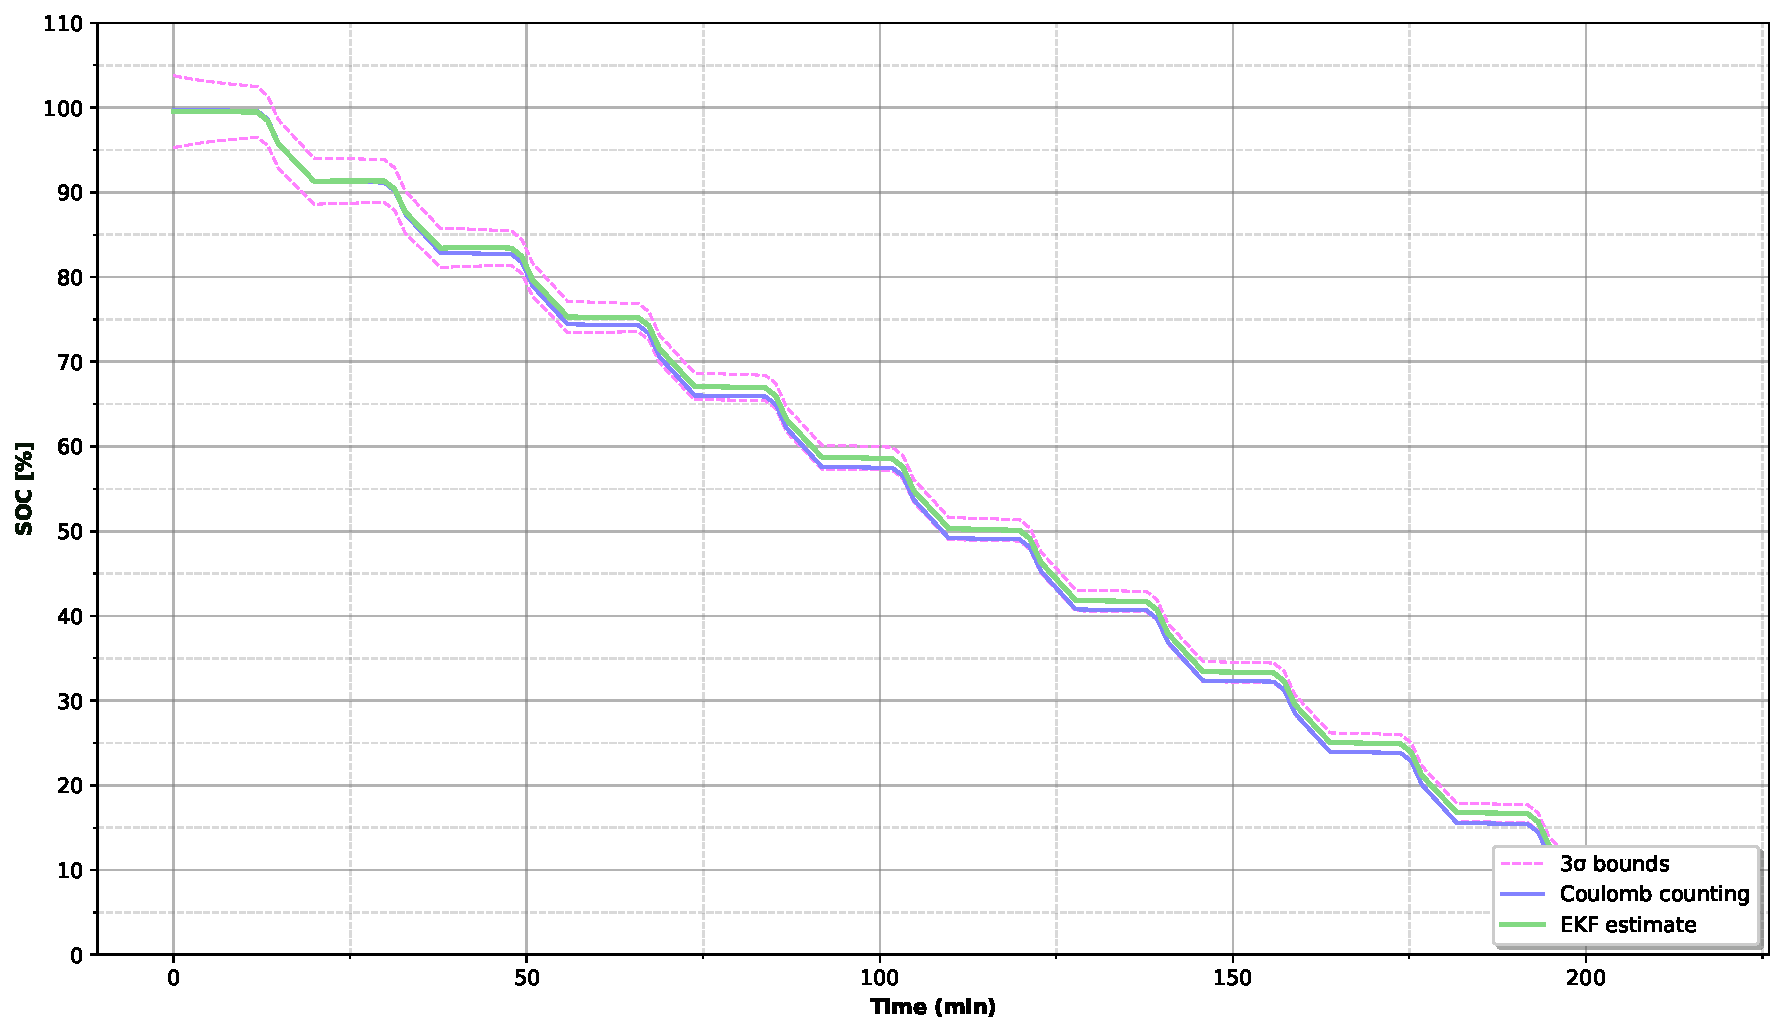
\includegraphics[width = 1\textwidth]{Codigo/Test Baterias/Battery_Graphs_Tests/EKF/dual/EKF_SOC_Steps_Test.pdf}
    \caption{SOC in time comparing Coulomb Counting method (lilac) and SOC \& SOH EKF estimator (green) during the random steps cycle of the \acs{NMC} battery.}
    \label{StepsEKFSOCSOHResults}
\end{figure}

The random step-current profile produced a \ac{SOC} \ac{RMSE} of $0.958\%$ (shown in Figures~\ref{StepsEKFSOCSOHResults} and~\ref{EStepsEKFSOCSOHErrorResults}). 

\begin{figure}[H]
    \centering
    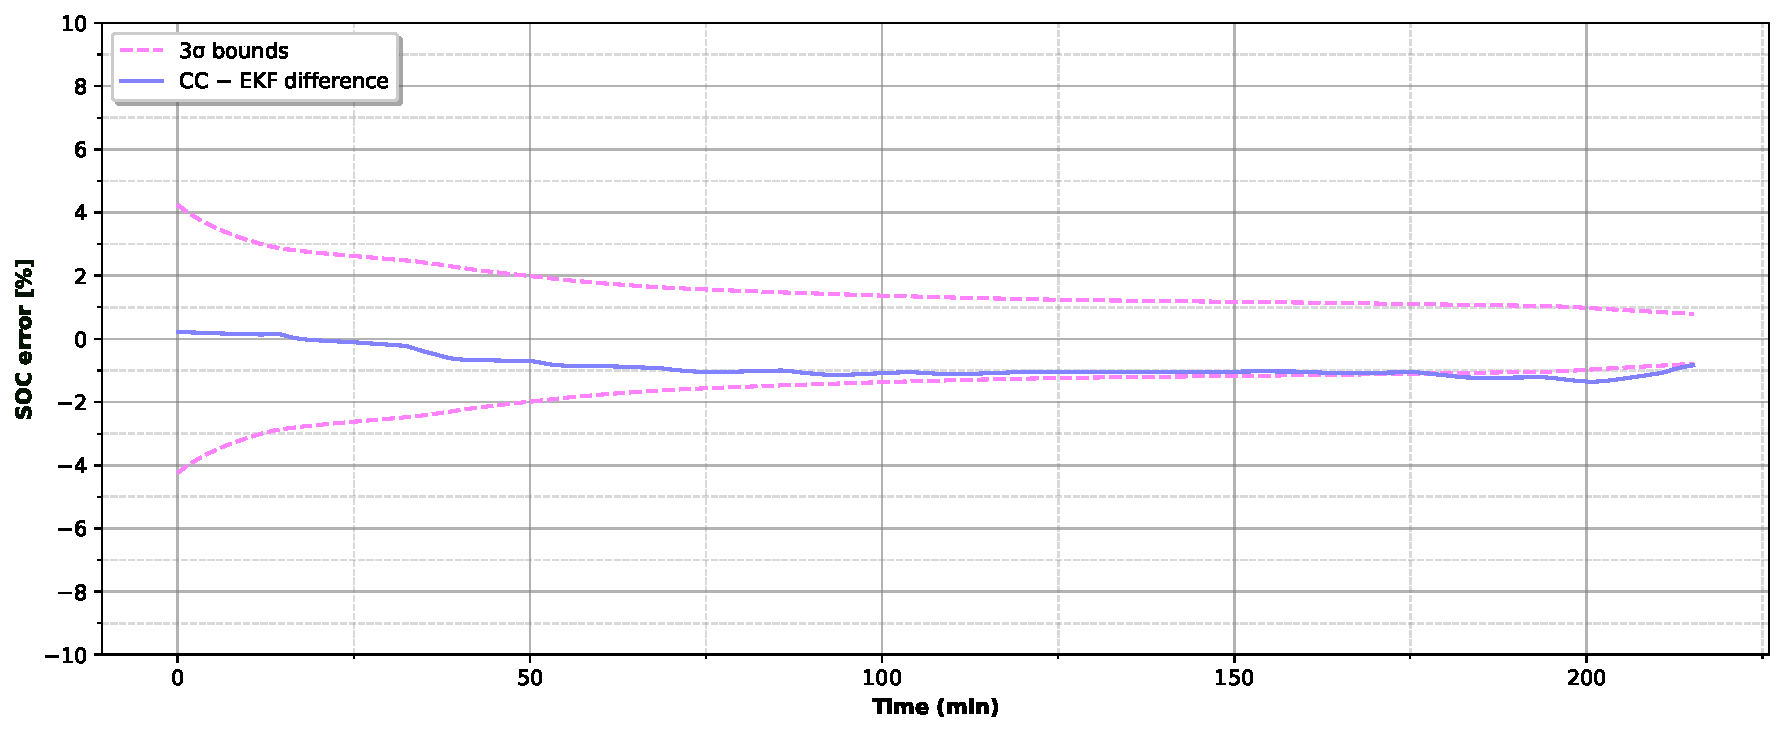
\includegraphics[width = 1\textwidth]{Codigo/Test Baterias/Battery_Graphs_Tests/EKF/dual/EKF_SOC_error_Steps_Test.pdf}
    \caption{Error between CC and dual EKF SOC estimator during the random steps cycle of the \acs{NMC} battery.}
    \label{EStepsEKFSOCSOHErrorResults}
\end{figure}

\subsection{Estimation Comparison between \acs{SOC} \& \acs{SOH} EKF and \acs{SOC} filter}

Figures~\ref{ChargeSOCComparisonResults},~\ref{PulsesSOCComparisonResults}, and~\ref{StepsSOCComparisonResults} 
directly compare the \acs{SOC} filter and dual \acs{EKF} estimates against the \acs{CC} reference. 
Although the dual filter's SOC RMSE was higher (as seen in 
Figures~\ref{ErrorChargeSOCComparisonResults},~\ref{ErrorPulsesSOCComparisonResults}, and~\ref{ErrorStepsSOCComparisonResults}), 
both estimators track the reference closely 
throughout the tests, confirming that the addition of simultaneous SOH estimation does not come at a significant cost to \acs{SOC} accuracy.

\begin{figure}[H]
    \centering
    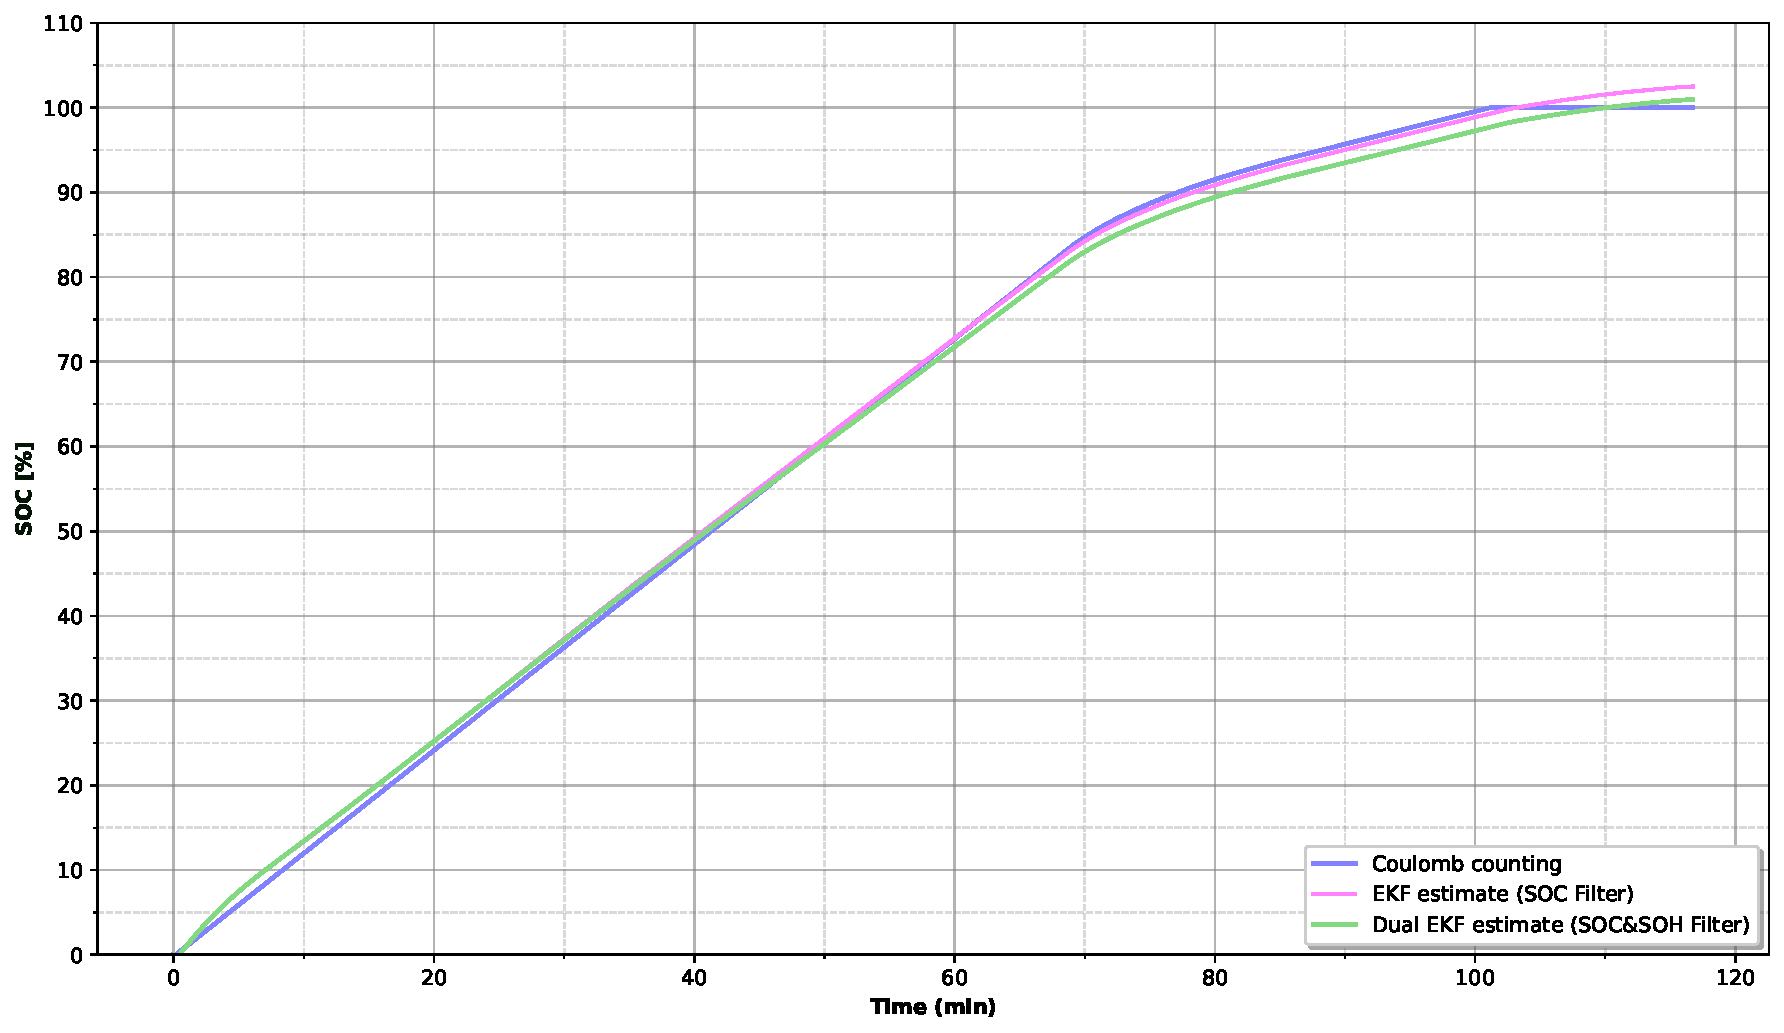
\includegraphics[width = 1\textwidth]{Codigo/Test Baterias/Battery_Graphs_Tests/EKF/comparison/EKF_SOC_comparison_Charge_Test.pdf}
    \caption{Comparison of \acs{SOC} estimation between the Coulomb-counting reference (lilac), 
    the \acs{SOC} \acs{EKF} filter (pink), and the \acs{SOC} \& \acs{SOH} \acs{EKF} (green) during the \acs{CC-CV} charging 
    cycle (constant-current phase at $20\,\text{A}$ up to approximately $70\,\text{min}$, 
    followed by the constant-voltage phase), sampled at $\Delta t = 1\,\text{s}$.}
    \label{ChargeSOCComparisonResults}
\end{figure}

\begin{figure}[H]
    \centering
    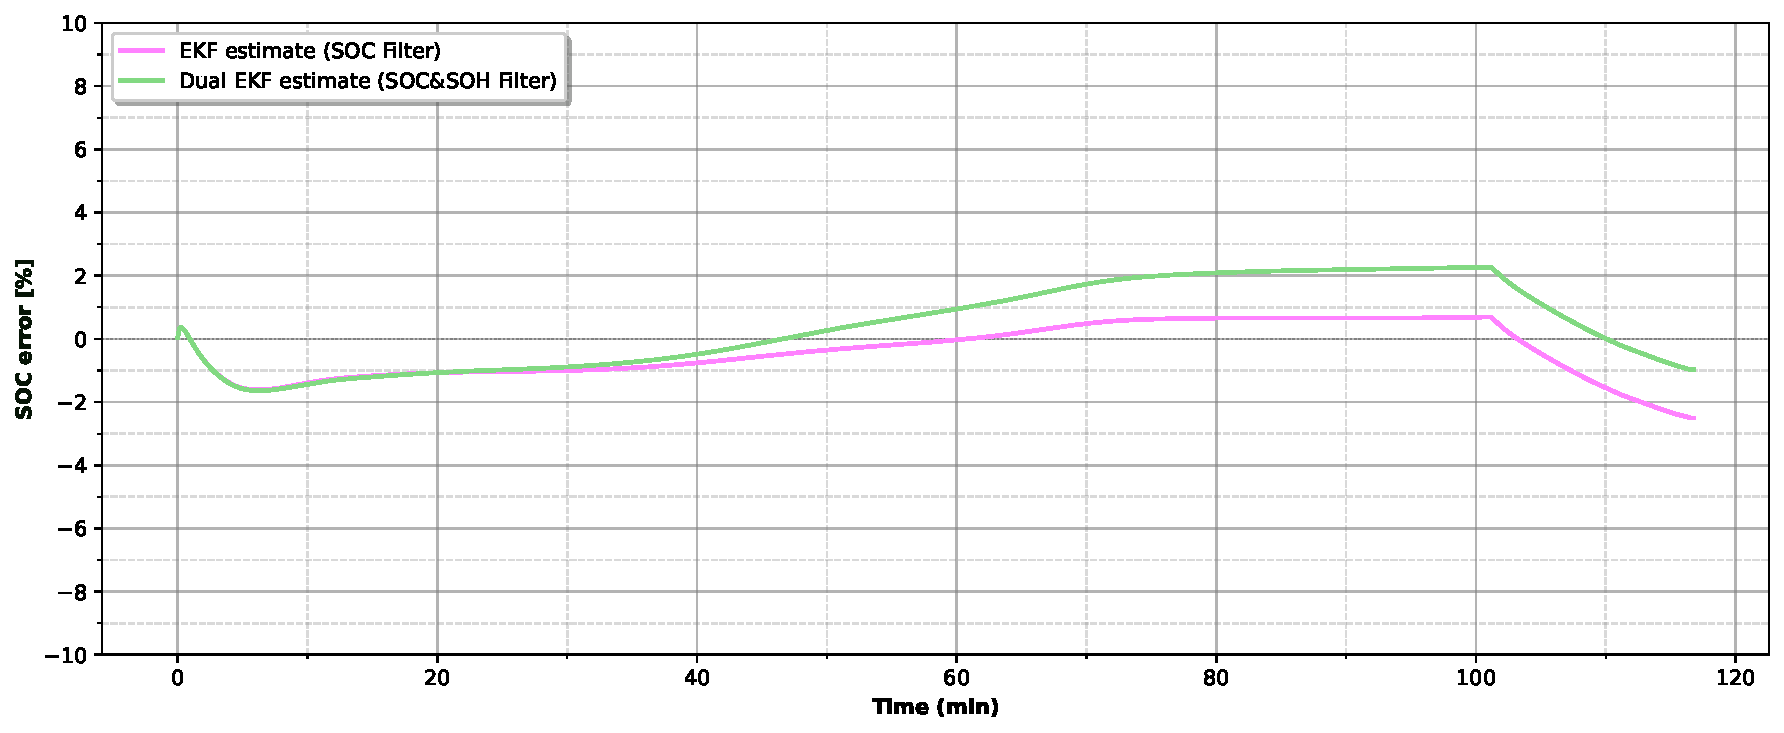
\includegraphics[width = 1\textwidth]{Codigo/Test Baterias/Battery_Graphs_Tests/EKF/comparison/EKF_SOC_error_comparison_Charge_Test.pdf}
    \caption{Comparison of Error between CC and 
    the \acs{SOC} \acs{EKF} filter (pink), and the \acs{SOC} \& \acs{SOH} \acs{EKF} (green) during the \acs{CC-CV} charging 
    cycle (constant-current phase at $20\,\text{A}$ up to approximately $70\,\text{min}$, 
    followed by the constant-voltage phase), sampled at $\Delta t = 1\,\text{s}$.}
    \label{ErrorChargeSOCComparisonResults}
\end{figure}

\begin{figure}[H]
    \centering
    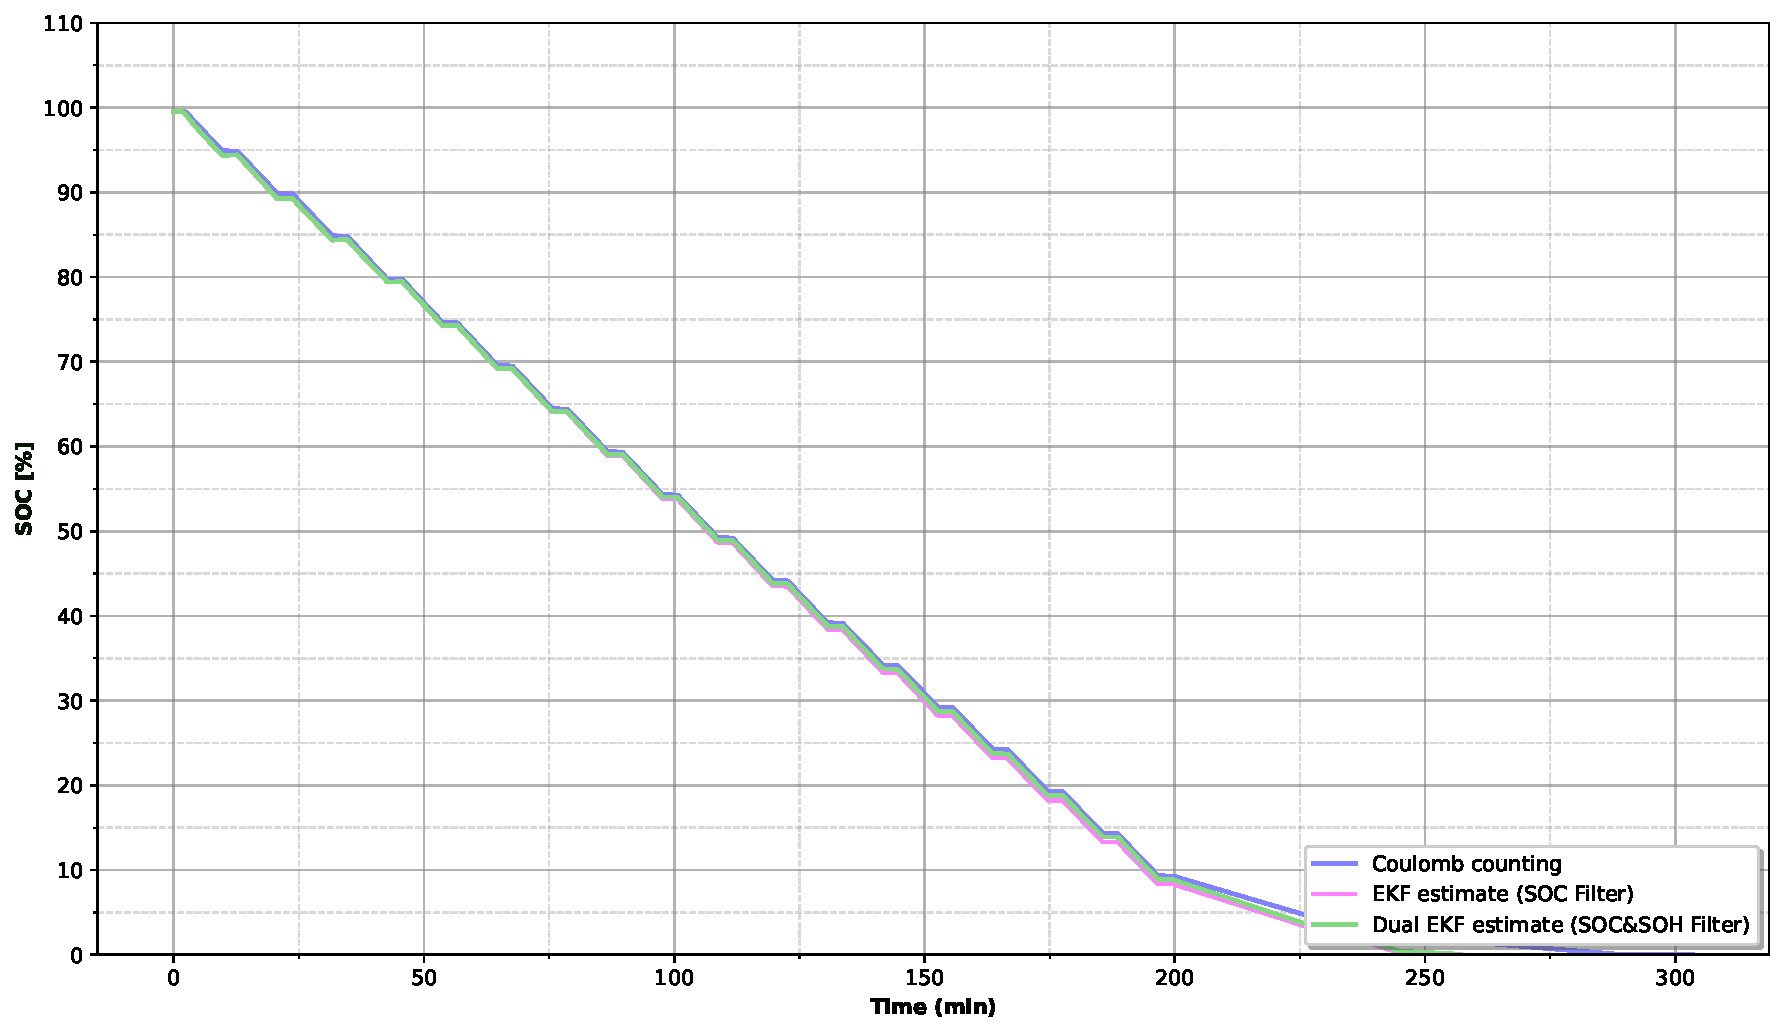
\includegraphics[width = 1\textwidth]{Codigo/Test Baterias/Battery_Graphs_Tests/EKF/comparison/EKF_SOC_comparison_Pulses_Test.pdf}
    \caption{Comparison of \acs{SOC} estimation between the Coulomb-counting reference (lilac), 
    the \acs{SOC} \acs{EKF} filter (pink), and the \acs{SOC} \& \acs{SOH} \acs{EKF} (green) during the cyclic pulse discharge of the \acs{NMC} 
    battery ($10\,\text{A}$ pulses of $10\,\text{min}$ separated by $3\,\text{min}$ 
    rest periods, until full discharge), sampled at $\Delta t = 1\,\text{s}$.}
    \label{PulsesSOCComparisonResults}
\end{figure}

\begin{figure}[H]
    \centering
    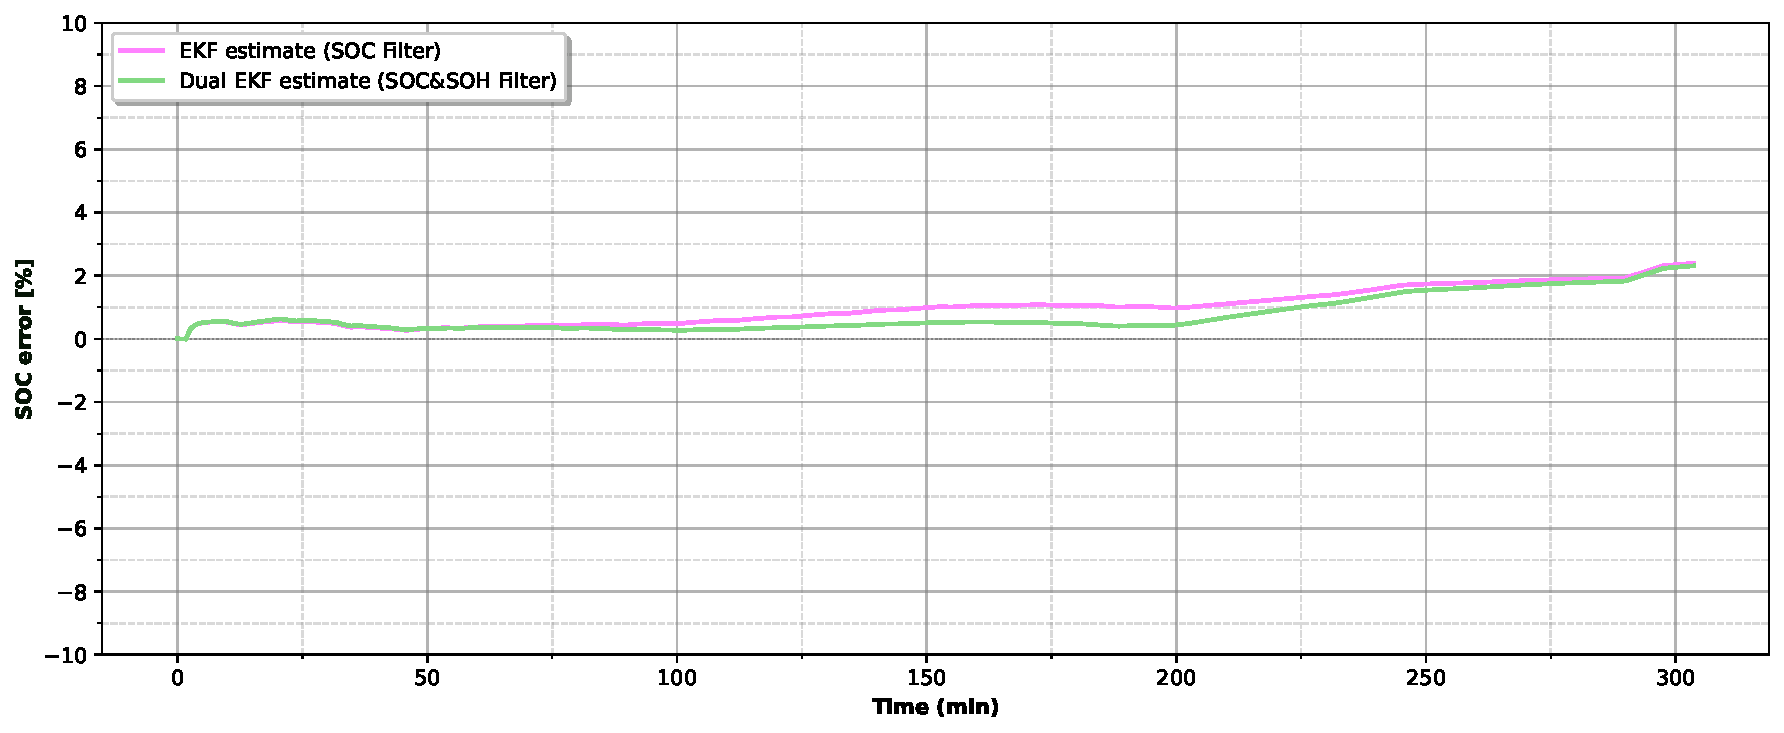
\includegraphics[width = 1\textwidth]{Codigo/Test Baterias/Battery_Graphs_Tests/EKF/comparison/EKF_SOC_error_comparison_Pulses_Test.pdf}
    \caption{Error between CC and 
    the \acs{SOC} \acs{EKF} filter (pink), and the \acs{SOC} \& \acs{SOH} \acs{EKF} (green) during the cyclic pulse discharge of the \acs{NMC} 
    battery ($10\,\text{A}$ pulses of $10\,\text{min}$ separated by $3\,\text{min}$ 
    rest periods, until full discharge), sampled at $\Delta t = 1\,\text{s}$.}
    \label{ErrorPulsesSOCComparisonResults}
\end{figure}

\begin{figure}[H]
    \centering
    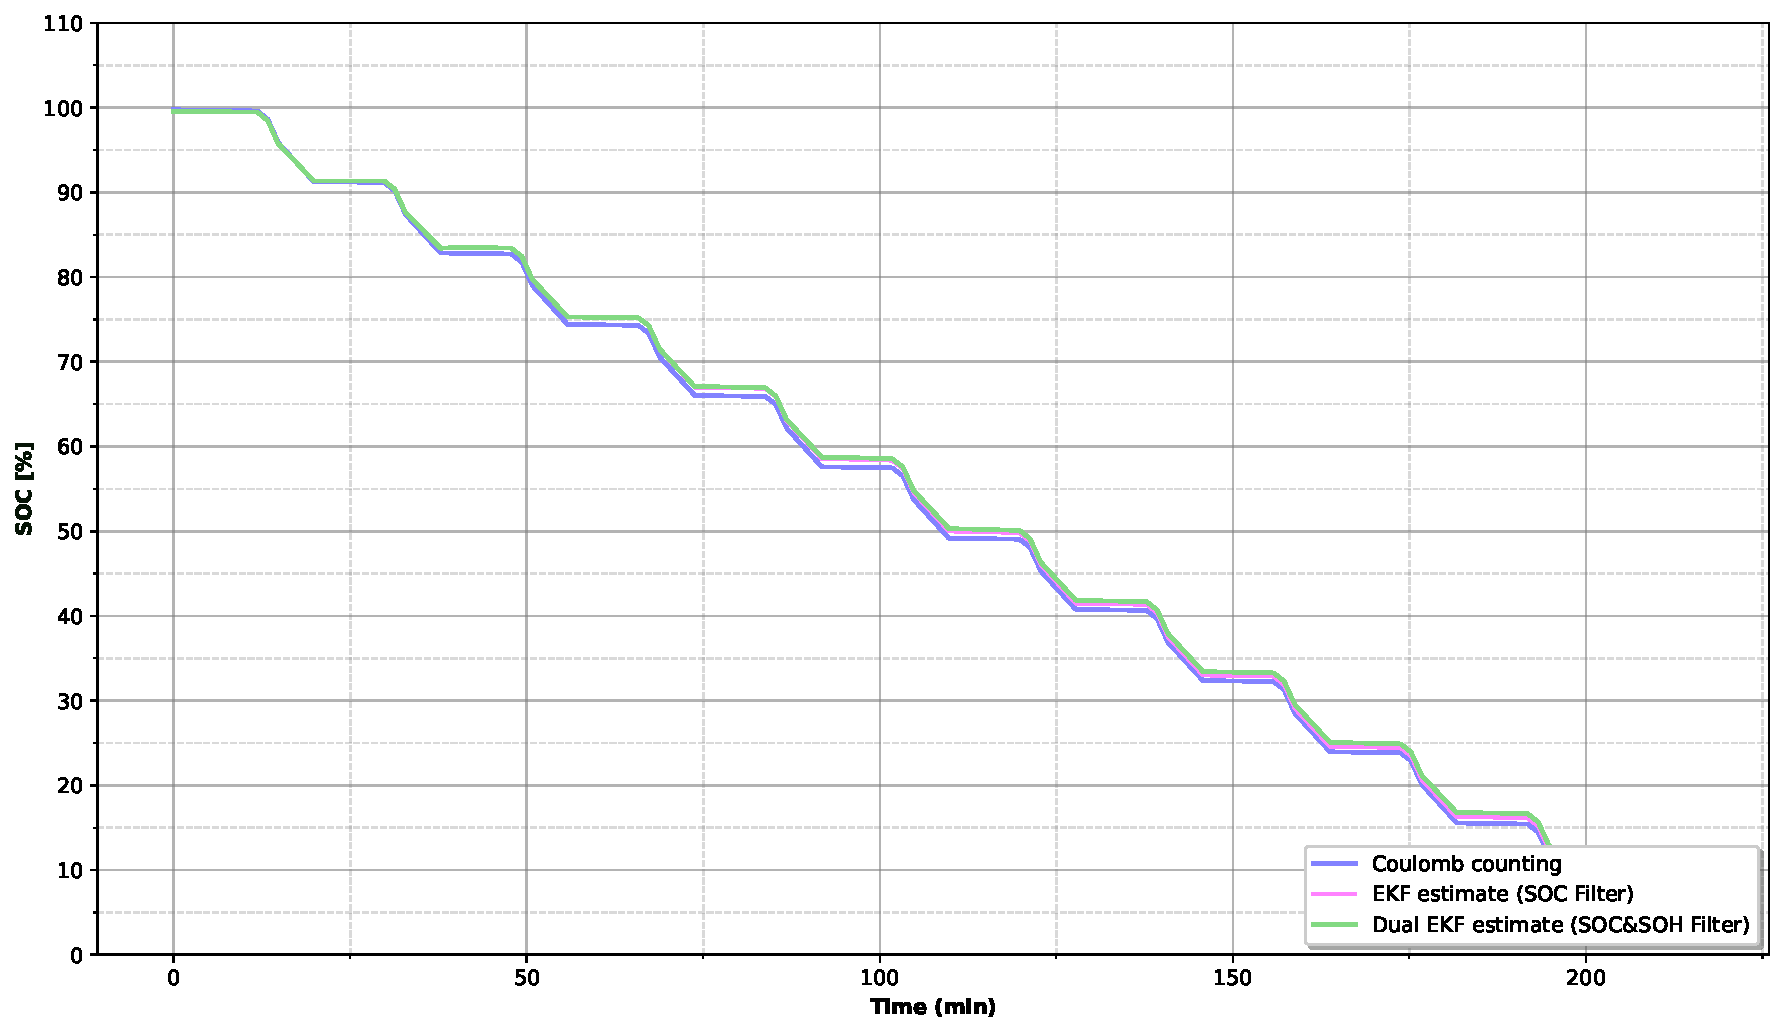
\includegraphics[width = 1\textwidth]{Codigo/Test Baterias/Battery_Graphs_Tests/EKF/comparison/EKF_SOC_comparison_Steps_Test.pdf}
    \caption{Comparison of \acs{SOC} estimation between the Coulomb-counting reference (lilac), 
    the \acs{SOC} \acs{EKF} filter (pink), and the \acs{SOC} \& \acs{SOH} \acs{EKF} (green) during the random step-current discharge of the 
    \acs{NMC} battery (steps between $0\,\text{A}$, $10\,\text{A}$, and $30\,\text{A}$), 
    sampled at $\Delta t = 1\,\text{s}$.}
    \label{StepsSOCComparisonResults}
\end{figure}

\begin{figure}[H]
    \centering
    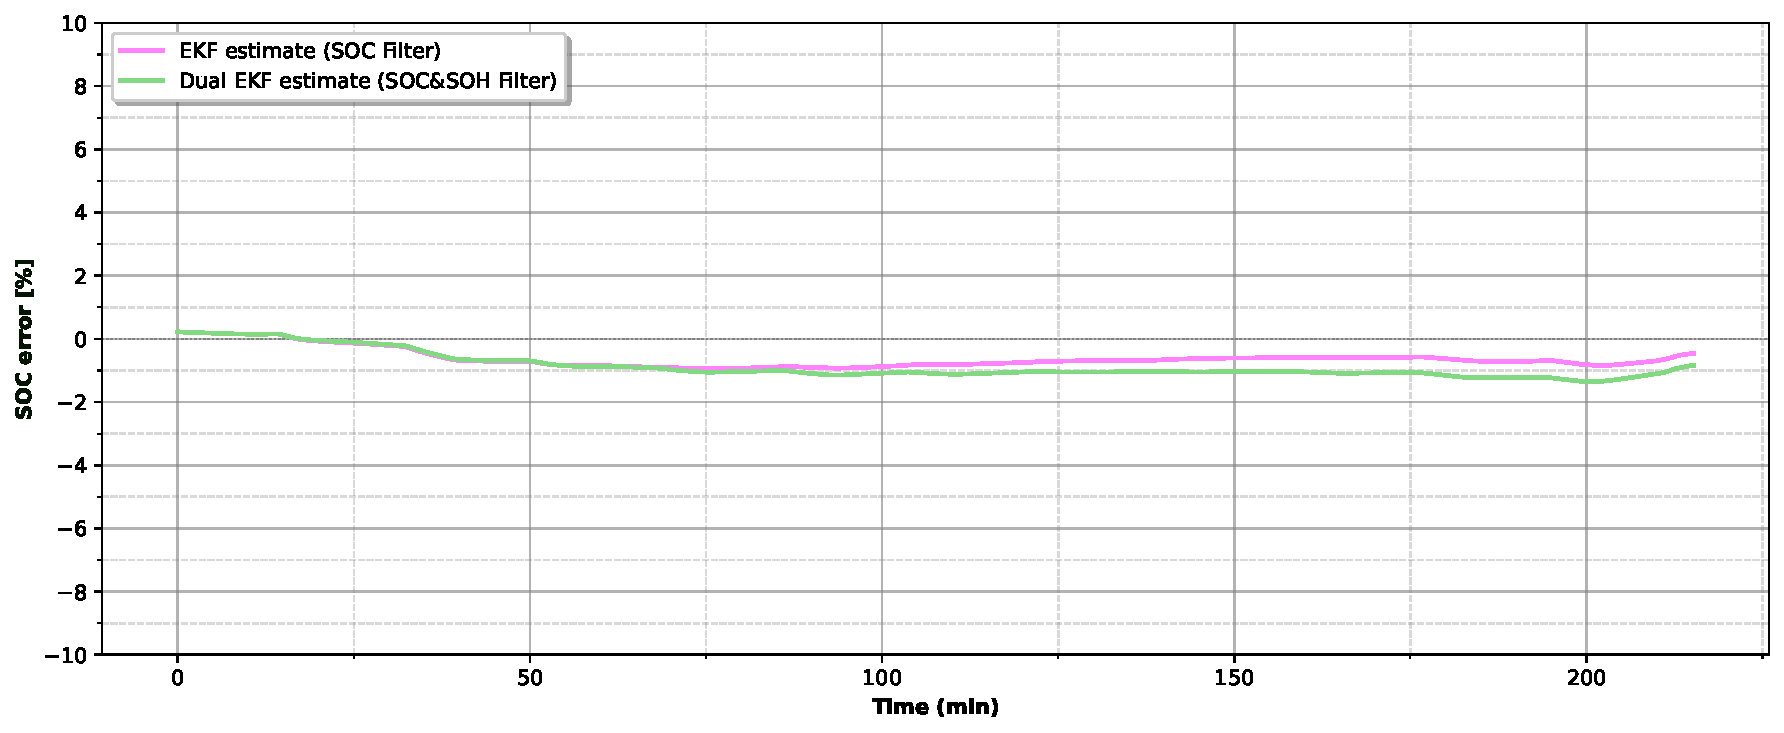
\includegraphics[width = 1\textwidth]{Codigo/Test Baterias/Battery_Graphs_Tests/EKF/comparison/EKF_SOC_error_comparison_Steps_Test.pdf}
    \caption{Error between CC and 
    the \acs{SOC} \acs{EKF} filter (pink), and the \acs{SOC} \& \acs{SOH} \acs{EKF} (green) during the random step-current discharge of the 
    \acs{NMC} battery (steps between $0\,\text{A}$, $10\,\text{A}$, and $30\,\text{A}$), 
    sampled at $\Delta t = 1\,\text{s}$.}
    \label{ErrorStepsSOCComparisonResults}
\end{figure}
